
\chapter{数学第三步，递归论}

递归论，或者也叫可计算性理论，创立于20世纪30年代，其研究内容就是两个方面：一是辨别某个特定的数学问题是否可以\underline{判定}(decide)，二是对于不可判定的问题，如何定量说明谁更复杂. 

我们首先看第一个问题，问题是否可判定. “判定”是一种\underline{能行过程}(effective procedure)，或者也称为\underline{算法}(algorithm)，当这个过程/算法结束以后，就要得出答案. 上面那些话说了跟没说一样，因为我们一直在引入新名词，但没有直白地解释这些名词. 什么是递归论？是研究问题是否可判定的理论. 什么是判定？是一个能行过程/算法. 什么是能行过程/算法？麻烦来了，这个问题没有精确答案，因为具体问题需要具体分析，而没有人知道所有问题的解决方法，只能泛泛地说，能行过程/算法是一套动作. 最著名的算法莫过于欧几里得《原本》中求两个自然数\(m,n\)的最大公约数的算法，这个算法用现代语言描述如下：
\begin{enumerate}
    \item 让\(m\)除以\(n\)，记\(r\)为余数（满足\(0\leq r < n\)）.
    \item 如果\(r=0\)，则\(n\)就是最大公约数，结束.
    \item 将\(m\)的值设为\(n\)，再将\(n\)的值设为\(r\)，回到第1步.
\end{enumerate}
观察这个算法，我们可以发现算法由有限多个步骤组成，我们总是从第1步开始执行，如果没有特别说明（比如“回到第1步”这类文字），就按顺序执行. 不过正是因为这类特别说明，我们要想学习一个算法，就不能像读小说一样囫囵地阅读，而要拿出纸笔亲自做一做. 尽管不能得出算法的定义，但我们能从这个例子中以小见大，归纳出算法的几个基本特征：
\begin{itemize}
    \item 有穷性(finiteness). 在执行有限多个步骤后会结束. 欧几里得这个算法满足这一点，虽然执行第3步后总要回到第1步，但每次回到第1步时\(n\)都比上次要小，因为余数\(r\)总小于\(n\)，而第3步将\(r\)的值赋给\(n\)，这就使得\(n\)越来越小，\(r\)也越来越小，\(r\)的值终将压到\(0\)，从而在第2步结束. 不能结束的程序不能称为算法，顶多称为计算方法(computational method)，比如计算圆周率小数点的程序，无限不循环小数，永远停不下来.
    \item 确定性(definiteness). 算法的每一步都是精确而直白的，就算没有相关知识积累的人，甚至是机器，也可以理解并执行. 欧几里得这个算法满足这一点，如果有哪里写得不太清楚的话，那只能说作者的语言文字功底还有待提高. 这一点菜谱是个反面教材，其中出现的语句诸如“加入小半勺盐”“翻面几次”“剁成小块”便是不精确的. 小半勺盐是多少克？对于碗口大的勺子200克也是小半勺；盐要加到哪里？加到中间也是加，撒在边上也是加. 或许这些指导对于大厨来说已经足够详细，但对于没有烹饪经验的人，或者是机器，这些描述还不够精确. 当然，确定性也是相对的.
    \item 能行性(effectiveness). 算法的每一步必须是能够做到的，最好是尽可能简单、尽可能基本. 欧几里得这个算法满足这一点，简单地做个除法和赋值，有纸笔就能做到，不能出现“对于正整数\(w,x,y,z,n\)，如果\(4\)是使得\(w^n+x^n+y^n=z^n\)能够成立的\(n\)的最大取值，那么跳至第3步”（哥德巴赫猜想）这类语句，也不能出现“将圆周率的每位小数依次代入”这类语句. 不过高阶图灵机这类模型，它可以一定程度上突破这点.
    \item 也许有输入，一定有输出. 我们在执行欧几里得这个算法之前给\(m,n\)指定了具体的值，这就是它的输入，而输出是最后的最大公约数.
\end{itemize}

初入递归论，都要求一切都建立在自然数上，讨论的数默认是自然数，讨论的函数默认定义在自然数上，讨论的命题/关系/谓词默认仅限于自然数. 借助哥德尔编码可以将有限长的序列/字符串/表达式与自然数一一对应，所以它们其实可以用同样的方法研究. 而字符串/表达式本身又可以用来描述更丰富集合——比如实数集和序数——的性质，我们便可以一层层套娃，把整个数学大厦都游览一遍. 如果函数对每个自然数都有定义，就称它是\underline{全函数}(total function)，否则就是\underline{部分函数}(partial function). 哪怕只讨论全函数，也并不都是可计算的：字符种类\(\Sigma\)是有限多的，描述算法的文字是有限长的，全体算法的集合的势是\({\rm card}(\Sigma^{<\omega})\)，而我们在朴素集合论里证明过，它小于\({\rm card}(\mathbb{N}^\omega)\)，所以实际上，绝大多数全函数都是不可计算的，因此可计算的函数就显得更为珍贵.

对于某个命题，如果存在一个算法判定它的真假，那就说这个命题是可判定的，而满足这个命题的所有东西组成的集合，就称为可判定集. 比如，偶数集就是可判定的集合，因为存在一个统一的算法判定一个数\(x\)是不是偶数：依次尝试比它小的数，如果其中一个数乘以2能得到\(x\)，那么\(x\)就是偶数. 同理，奇数集可判定，素数集可判定，斯特林数集可判定，欧拉数集可判定，等等等，我们能想到的集合，大多都是可判定的，不可判定的集合反而没那么容易想到，比如全体有关于自然数的命题组成的集合（后面我们会证明）.

由于不能给算法下准确的定义，因此也没办法准确刻画所谓\underline{直观可计算}(effectively calculable)的性质——毕竟“直观”一词就十分玄妙. 也许对于某些比较典型的函数，我们可以从直觉上判断它是不是直观可计算的，但想要从个性中准确归纳出共性，从而明确直观可计算与直观不可计算的边界，是没法做到的. 历史上人们多次尝试刻画可计算性，比较经典的有哥德尔和克林尼定义的递归函数、丘奇定义的Lambda可定义函数、图灵定义的图灵可计算函数、波斯特定义的典范演绎系统函数、马可夫的基本字符集算法等，非常巧的是，这些刻画恰好是等价的，可以说它们都把握住了直观可计算的精髓. 接下来介绍前三种，关于此，丘奇和图灵有两个比较重要的论断.

\begin{reference}
    丘奇论题(Church thesis)：直观上可计算的函数就是Lambda可定义函数.\newline
    丘奇-图灵论题(Church-Turing thesis)：直观上可计算的函数就是图灵可计算函数.
\end{reference}

因为人们说不清楚直观可计算函数长什么样，所以这两个论题只能称为论题而非定理，其实这两个论题更像是一种宣称，断言自己的构造足以刻画“直观可计算”性质了. 虽然人们有理由相信这几种等价的可计算性就是人们直观上的可计算性，并且未来可计算性理论的发展也可能不断检验并支撑这一点，但却没有办法证明这一点，因为谁也不知道直观上的可计算性究竟是个什么样子，谁也不能绝对地保证将来不会出现这七种等价的可计算性概念无法把握的直观上可计算的函数。

\section{递归函数}

\subsection{原始递归函数}

递归函数是对可计算函数的一种刻画尝试
\begin{definition}{原始递归函数}
    以下记\(\vec x\)为“\(x_1,x_2,\cdots,x_n\)”的简写. 初始函数有三类.
    \begin{itemize}
        \item 常函数. \(C^n_k(\vec x) = k\)，上标\(n\)表示其是\(n\)元函数.
        \item 投影函数. \(P^n_i(\vec x) = x_i\)，上标\(n\)表示其是\(n\)元函数.
        \item 后继数函数. \(S(x) = x+1\).
    \end{itemize}
    原始递归函数有三个来源.
    \begin{itemize}
        \item 初始函数是原始递归函数.
        \item （复合）设\(h\)是\(m\)元递归函数，\(g_1,\cdots,g_m\)是\(m\)个\(n\)元原始递归函数，则
        \[f(\vec x) = h(g_1(\vec x),g_2(\vec x),\cdots,g_m(\vec x))\]
        也是一个\(n\)元原始递归函数，此时记\(f=h\circ(g_1,g_2,\cdots,g_m)\).
        \item （归纳）设 \(g\)是\(n\)元原始递归函数，\(h\)是\(n+2\)元原始递归函数，若\(n+1\)元函数\(f\)按如下归纳定义
        \begin{align*}
            f(0,\vec x) &= g(\vec x) \\
            f(n+1,\vec x) &= h(n,f(n,\vec x),\vec x)
        \end{align*}
        则\(f\)是由\(g,h\)归纳出的原始递归函数，记作\(f=\rho(g,h)\).
    \end{itemize}
\end{definition}

我们所能见到的\(\mathbb{N}^n \to \mathbb{N}\)的各种函数和运算符，很多都是原始递归函数，举几个例子.
\begin{itemize}
    \item 加法. 大家知道，加法的定义是
    \[x+0 = x\]
    \[x+S(y)=S(x+y)\]
    把加号写成函数的形式，记\({\rm add}(x,y)=x+y\)，观察这两条定义，这明显是归纳的形式，即存在两个函数\(g,h\)使得
    \[{\rm add}(0,x)=g(x)\]
    \[{\rm add}(S(y),x)=h(y,{\rm add}(y,x),x)\]
    对比一下这两组式子，不难看出，\(g(x)=P^1_1(x)\)，\(h(x_1,x_2,x_3)=S(x_2)=S(P^3_2(x_1,x_2,x_3))\)，因此\({\rm add}=\rho(P^1_1,S\circ P^3_2)\)

    \item 乘法. 大家也知道，乘法的定义是
    \[x \cdot 0 = x\]
    \[x \cdot S(y) = x + x \cdot y\]
    把乘号写成函数的形式，记\({\rm mul}(x,y)=x \cdot y\)，观察这两条定义，这明显又是归纳的形式，即存在两个函数\(g,h\)使得
    \[{\rm mul}(0,x)=g(x)\]
    \[{\rm mul}(S(y),x)=h(y,{\rm mul}(y,x),x)\]
    对比一下这两组式子不难看出，\(g(x)=C^1_0(x)\)，而
    \[h(x_1,x_2,x_3)={\rm add}(x_3,x_2)={\rm add}(P^3_3(x_1,x_2,x_3),P^3_2(x_1,x_2,x_3))\]
    因此\({\rm mul} = \rho(C^1_0,{\rm add} \circ (P^3_3,P^3_2)) = \rho(C^1_0,\rho(P^1_1,S\circ P^3_2) \circ (P^3_3,P^3_2))\)

    \item 乘方. 大家还知道，乘方的定义是
    \[x^0 = 1\]
    \[x^{S(y)} = x \cdot x^y\]
    写成函数的形式，记\({\rm exp}(x,y)=x^y\)，观察这两条定义，这明显又是归纳的形式，即存在两个函数\(g,h\)使得
    \[{\rm exp}(0,x)=g(x)\]
    \[{\rm exp}(S(y),x)=h(y,{\rm exp}(y,x),x)\]
    对比一下这两组式子不难看出，\(g(x)=C^1_1(x)\)，而
    \[h(x_1,x_2,x_3)={\rm mul}(x_3,x_2)={\rm mul}(P^3_3(x_1,x_2,x_3),P^3_2(x_1,x_2,x_3))\]
    因此\({\rm exp}=\rho(P^1_1,{\rm mul} \circ (P^3_3,P^3_2)) = \rho(P^1_1,\rho(C^1_0,\rho(P^1_1,S\circ P^3_2) \circ (P^3_3,P^3_2)) \circ (P^3_3,P^3_2))\)

    \item 阶乘. 大家继续知道，阶乘的定义是
    \[0!=1\]
    \[S(x)! = S(x) \cdot x!\]
    这明显还是归纳的形式，即存在两个函数\(g,h\)使得
    \[0!=g(x)\]
    \[S(x)!=h(x,x!)\]
    对比一下这两组式子不难看出，\(g(x)=C^1_1(x)\)，而
    \[h(x_1,x_2)={\rm mul}(S(x_1),x_2) = {\rm mul}(S(P^2_1(x_1,x_2),P^2_2(x_1,x_2)))\]
    所以\(\cdot !=\rho(C^1_1,\rho(P^1_1,\rho(P^1_1,S\circ P^3_2) \circ (P^3_3,P^3_2)) \circ (S \circ P^2_1,P^2_2))\)

    \item 有界前行函数(predecessor)，和后继数刚好反过来，\({\rm prec}(x)=x-1\)（不是定义式）. 因为现在只讨论自然数，所以这里要补充定义\({\rm prec}(0)=0\). 乍一看不知道怎么拼凑，但实际上只要注意到\({\rm prec}(S(x))=x\)，就可以发现其实还是老套的归纳. 即存在两个函数\(g,h\)使得
    \[{\rm prec}(0)=g(x)\]
    \[{\rm prec}(S(x))=h(x,{\rm prec}(x))\]
    不难看出，\(g(x)=C^1_0(x)\)，\(h(x_1,x_2)=x_1 = P^2_1(x_1,x_2)\)，所以\({\rm prec} = \rho(C^1_0, P^2_1)\)
    
    \item 有界减法. 和加法刚好反过来，在自然数上讨论问题，也要补充定义，当\(x<y\)时\(x-y=0\). 需要注意，“\(<\)”这个关系成立与否的判断过程到底是不是原始递归的，现在还没有证明，所以现在不用大于小于号来定义自然数减法，而用已经证明是原始递归的前行函数来定义：
    \[x-0 = x\]
    \[x-S(y) = {\rm prec}(x-y)\]
    写成函数的形式，记\({\rm sub}(x,y)=x-y\)，这明显还是归纳的形式，即存在两个函数\(g,h\)使得
    \[{\rm sub}(x,0)=g(x)\]
    \[{\rm sub}(x,S(y))=h(y,{\rm sub}(x,y),x)\]
    不难看出，\(g(x) = P^1_1(x)\)，\(h(x_1,x_2,x_3)={\rm prec}(x_2) = {\rm prec}(P^3_2(x_1,x_2,x_3))\)，因此\({\rm sub} = \rho(P^1_1, \rho(C^1_0, P^2_1) \circ P^3_2)\).
    
\end{itemize}

在朴素集合论里提到，运算符可以看作函数，而函数又是一种特殊的关系/谓词. 但在递归论中，函数才是老大，判断某个关系/谓词成立与否的过程是不是原始递归的，要借助示性函数.

\begin{definition}{原始递归关系}
    对于装备在\(\mathbb{N}\)上的关系\(P\)，其示性函数
    \[\chi_P(\vec x) = \left\{\begin{aligned}
        &1, &&P(\vec x)\mbox{成立} \\
        &0, &&P(\vec x)\mbox{不成立}
    \end{aligned}\right.\]
    如果是原始递归的，那么就称关系\(P(x)\)是原始递归的，集合\(\{x \in \mathbb{N}| P(x)\}\)是原始递归集.
\end{definition}

这是一个比较绕的地方，联系朴素集合论，对于一元关系，\(P(x)\)成立即\(x \in P\)，而原始递归集\(\{x \in \mathbb{N} | P(x)\} = \{x \in \mathbb{N} | x \in P\}\)，如果我们默认论域就是\(\mathbb{N}\)，那么又等于\(\{x| x \in P\}\)，即\(P\)自己. 所以对于一元关系\(P \in \mathbb{N}\)，说\(P\)是原始递归关系，和说\(P\)是原始递归集是同一个意思. 接下来举几个例子.
\begin{itemize}
    \item 关系\footnote{这里将关系和谓词混用，如果严格地区分两者，从谓词的角度来看\({\rm zero}(x): x=0\)表示自然数模型\(\mathcal{N} \vDash {\rm zero}[0]\)且对于其他自然数\(n\)有\(\mathcal{N} \not\vDash {\rm zero}[n]\)；如果从关系的角度来看\({\rm zero} = \{x | x=0\} = \{0\}\)}\({\rm zero}(x): x=0\)是原始递归的. 记其示性函数为\(\chi_{\rm zero}\)，有\(\chi(0)=1,\chi(S(x))=0\)，归纳呗，\(\chi_{\rm zero} = \rho(C^1_1,C^2_0)\). 同理\({\rm pos}(x): x > 0\)也是原始递归的，因为\(\chi_{\rm pos}(x) = \rho(C^1_0,C^2_1)\).
    \item 关系\({\rm leq}(x,y):x \leq y\)是原始递归的. 记其示性函数为\(\chi_\leq\)，因为\(x \leq y \Longleftrightarrow x-y = 0 \Longleftrightarrow \chi_{\rm zero}(x-y)=1\)，因此\(\chi_\leq = \chi_{\rm zero} \circ {\rm sub} = \rho(C^1_1,C^2_0) \circ \rho(P^1_1, \rho(C^1_0, P^2_1) \circ P^3_2)\).
    \item 关系\({\rm equ}(x,y): x=y\)是原始递归的，记其示性函数为\(\chi_=\)，因为\(x = y \Longleftrightarrow (x \leq y\mbox{且}y \leq x)\)，所以\(\chi_=(x,y) = \chi_\leq(x,y) \cdot \chi_\leq(y,x)\)，再把乘法代入即
    \[\chi_= = \rho(P^1_1,\rho(P^1_1,S\circ P^3_2) \circ (P^3_3,P^3_2)) \circ (\rho(C^1_1,C^2_0) \circ \rho(P^1_1, \rho(C^1_0, P^2_1) \circ P^3_2),\rho(C^1_1,C^2_0) \circ \rho(P^1_1, \rho(C^1_0, P^2_1) \circ P^3_2))\]
    \item （复合）设\(P\)是\(m\)元原始递归关系，\(g_1,g_2,\cdots,g_m\)是原始递归函数，则
    \[Q(\vec x) = P(g_1(\vec x), g_2(\vec x), \cdots, g_n(\vec x))\]
    也是原始递归关系. 因为\(\chi_Q(\vec x) = \chi_P \circ (g_1,g_2,\cdots,g_n)\).
    \item （集合的基本操作）设\(P,Q\)都是\(n\)元原始递归关系，则\(\bar P = \mathbb{N}^n - P\)也是原始递归关系，\(P \cup Q, P \cap Q\)也是原始递归关系. 因为\(\chi_{\bar P} = \chi_{\rm zero} \circ \chi_P\)，\(\chi_{P \cup Q} = {\rm pos}(\chi_{P} + \chi_{Q})\)，\(\chi_{P \cap Q} = \chi_P \cdot \chi_Q\).
    \item （分情况定义）数学里很多函数是分情况定义的，就拿两种情况举个例子，形如
    \[f(\vec x) = \left\{ \begin{aligned} &g_1(\vec x), &\mbox{如果}P(\vec x)\mbox{成立} \\ &g_2(\vec x), &\mbox{否则} \end{aligned} \right.\]
    如果\(g_1,g_2,P\)都是原始递归的，那么\(f\)也是原始递归的，因为\(f = g_1\chi_P+g_2\chi_{\bar P}\). 类似地，更多种情况也是如此.
    \item （有界成立定义）设\(P(\vec x, y)\)是原始递归关系，则
    \[Q = \{(\vec x, y) | \mbox{对于任意}t<y\mbox{都有}(\vec x, t) \in P\}\]
    可以简记为\(Q = \{(\vec x, y)|(\forall t < y)P(\vec x,t)\}\)，也是原始递归关系，因为\(\displaystyle{\chi_Q(\vec x, y) = \prod_{t \leq y}\chi_P(\vec x,t)}\)，是有限多个东西相乘. 同理
    \[Q = \{(\vec x, y) | \mbox{存在}t<y\mbox{使得}(\vec x, t) \in P\}\]
    可以简记为\(Q = \{(\vec x, y)|(\exists t < y)P(\vec x,t)\}\)，也是原始递归关系，因为\(\displaystyle{\chi_Q(\vec x, y) = {\rm pos}\left(\sum_{t \leq y}\chi_P(\vec x,t)\right)}\)，是有限多个东西相加再复合.
\end{itemize}

\subsection{极小算子}

计算机程序能干很多事情，以上所说的原始递归函数都可以用计算机程序来实现，初始函数不用说了，原始递归函数的复合在计算机程序里也体现为函数的复合，分情况定义体现为\lstinline|if...else...|语句块（分支结构），原始递归函数的归纳则体现为\lstinline|for|循环（指定次数循环）. 但是计算机程序里的\lstinline|while|循环（指定条件循环）在原始递归函数里并没有对应的东西，于是我们现在引入极小算子.

\begin{definition}{极小算子}
    记\(\vec x\)为“\(x_1,x_2,\cdots,x_n\)”的简写，设\(P(\vec x,y)\)是装备在\(\mathbb{N}\)上的多元关系，当参数\(\vec x\)固定时，最小的、能使得\(P(\vec x,y)\)成立的参数\(y\)就记为\(\mu yP(\vec x,y)\).
\end{definition}

看起来比较抽象，有必要好好解释，我们曾经举例，以下几个常见的算符会“约束”变量\(x\)，使其变成“哑变量”：
\[\sum_{x=\cdots} \qquad \prod_{x=\cdots} \qquad \int \cdots {\rm d}x \qquad \lim_{x \to \cdots} \qquad \forall x \qquad \exists x\]
现在要增加一个算符，就是极小算符\(\mu\). 而表达式\(\mu yP(\vec x,y)\)是一个数，是什么数呢？是当\(\vec x\)固定时使得\(P(\vec x,y)\)成立的的最小的数，用集合论语言改写就是
\[\mu y P(\vec x,y) = \min\{y \in \mathbb{N}|P(\vec x,y)\}\]

那么，这个极小算子如何体现\lstinline|while|循环呢？举个具体的例子，如果关系\(P(x_1,x_2,x_3 ,y)\)是已知的，定义函数
\[f(x_1,x_2,x_3) = \mu y P(x_1,x_2,x_3, y)\]
比如现在想求\(f(8,8,8)\)是多少，就要先代入\(y=0\)，看看\(P(8,8,8,0)\)是否成立，如果成立的话，\(f(8,8,8)=0\)；如果不成立，再代入\(y=1\)，如果\(P(8,8,8,1)\)成立的话，\(f(8,8,8)=1\)；如果不成立，再代入\(y=2\)……将\(y\)从小到大遍历每个自然数，直到\(P\)成立，此时的\(y\)值就是\(f\)的函数值. 这就体现了指定条件循环的思想. 递归论是和计算机编程结合得非常紧密的数学分支，我们可以将例子中的函数\(f\)以代码的形式表现出来.

\begin{lstlisting}[language = Python]
def f(x1,x2,x3):
    y = 0
    while not P(x1,x2,x3,y): y += 1
    return y
\end{lstlisting}

万一\(P(8,8,8,y)\)对所有\(y\)都不成立呢？那\(f(8,8,8)\)就是未定义的，或者称其是发散的，没有值，此时记作\(f(8,8,8)\uparrow\)，同理，如果我们想笼统地表示\(f(8,8,8)\)不是发散的，就写作\(f(8,8,8)\downarrow\). 

\begin{definition}{递归函数}
    \underline{递归函数}(general recursive function)有两个来源.
    \begin{itemize}
        \item 原始递归函数是递归函数.
        \item （极小化）设\(g(\vec x,y)\)是递归函数，则\(f(\vec x)=\mu y (g(\vec x, y)=0)\)也是递归函数\footnote{\(\mu y. (g(\vec x, y)=0)\)的意思是使得\(g(\vec x,y)=0\)成立的最小的\(y\)，同时对小于这个\(y\)的任意自然数\(z\)，\(g(\vec x,z)\)都必须有定义，这点很重要，否则会产生非递归的函数.}.
    \end{itemize}
\end{definition}

我们也可以说，递归函数就是初始函数经由有限次复合、归纳和极小化得到的函数. 极小化之所以有别于复合与归纳，就在于它可能会产生无定义的点，因为\(g(\vec x, y)\)可能无论对哪个\(y\)都大于\(0\)，但复合与归纳没有这个问题. 进一步说，要想知道某个点究竟有没有定义，如果给定了具体的函数，那倒是可以具体分析，但是就从最一般的递归函数层面来说，不存在一个统一的算法判定某个函数的某个点是否有定义.

虽然极小算子会产生非原始递归但递归的函数，但如果令极小算子的搜索限定在一个有限的范围内，比如小于某个数\(z\)，那就无法突破原始递归函数的藩篱. 这样的极小算子称为有界极小算子(bounded minimalization).

\begin{proposition}{}
    对于原始递归函数\(g(\vec x,y)\)，\(f(\vec x) = (\mu y \leq z)(g(\vec x,y)=0)\)也是原始递归函数.
\end{proposition}

\subsection{哥德尔编码}

本节要介绍的哥德尔编码，内容不多，却是贯穿集合论、递归论、证明论、模型论的重量级工具. 其思想是构造一个单射，把形式语言（包括前面学的逻辑语言和演算语言）中的表达式对应为某个自然数，这个过程称为\underline{编码}(encode)；反过来，对于某个自然数，如果它在该单射的值域内，我们也可以很快地（原始递归地）反推出该自然数由哪个表达式编码而来，这个反推的过程称为\underline{解码}(decode). 有了编解码这个工具，我们就可以使用算术的方法来研究表达式的性质. 

编解码的可行性，或者该单射的存在性，我们早已在朴素集合论中证明了. 如果符号字典\(\Sigma\)是有限的，则\({\rm card}(\Sigma^{<\omega}) = {\rm card}(\mathbb{N})\)，即有限长表达式的集合可以与自然数建立双射.

\begin{definition}{哥德尔编码}
    设有字典\(\Sigma\)，给每个元素都编号. 对于序列\(\{a_1,a_2,\cdots,a_n\}\)，\(a_i\)的编号记为\(\# a_i\)，则
    \[\#(a_1,a_2,\cdots,a_n) := 2^{1+\#a_1}3^{1+\#a_2}\cdots p_n^{1+\#a_n}\]
    为序列的\underline{哥德尔数}(Gödel number)，其中\(p_n\)是第\(n\)个素数. 如果是空序列，规定\(\#()=1\). 
\end{definition}

该定义把字符串编码成了自然数，现在要反过来，将自然数解码成原来的字符串，这就是纯数论的内容了. 首要需要明确字符串有多长，哥德尔数\(x\)是多个素数相乘，如果字符串长度为\(n\)，那么参与相乘的最大素数是\(p_n\)，所以素数\(p_1\)到\(p_n\)都可以整除\(x\)但\(p_{n+1}\)不行，于是我们约定
\[{\rm len}(x) = (\mu k < x)(\neg \exists m(mp_{k+1}=x)), \qquad {\rm len}(1) = 0\]
从自然数\(x\)反求序列长度. 同理，如果第\(i\)项的编号是\(n\)，那么\(p_i, p_i^2, \cdots, p_i^n\)都可以整除\(x\)但\(p_i^{n+1}\)不行，所以我们约定
\[(x)_i = (\mu k < x)(\neg \exists m(mp^{k+2}=x))\]
从自然数\(x\)中反求序列第\(i\)项的编号. 项数既可以从\(1\)开始算起也可以从\(0\)算起，如果从\(1\)算起就不关心\((x)_0\)的定义，但此时为了保证\((x)_i\)是全函数，可以补充规定\((x)_0=0\).

以上，“\(\#\)”给元素及其序列编码为自然数，而“\({\rm len}(x), (x)_i\)”则把自然数解码为原序列，难能可贵的是，\textbf{编解码的过程都是原始递归的}，这个性质极其重要，在集合论、递归论、证明论中都有所应用，观察这三个家伙的形式，容易判断解码所用到的两个函数是原始递归的，现在只需要证明素数枚举函数\(p_n\)也是原始递归的就好了.
\begin{itemize}
    \item 关系“\(y\)能被\(x\)整除”（或者说“\(y\)是\(x\)的整数倍”，记作\(x|y\)）是原始递归关系，因为\(x|y: (\exists n < y)(n\cdot x = y)\)，是有界成立定义.
    
    \item “\(D(x) := x\)的因数个数”是原始递归函数，因为如果记关系“\(y\)能被\(x\)整除”的示性函数为\(\chi_{\rm div}(x,y)\)，则
    \[D(x) = \sum_{k=1}^{n} \chi_{\rm div}(k,x)\]
    因此我们可以进一步断言，关系“\(x\)是素数”是原始递归关系，因为它的示性函数
    \[\chi_{\rm prime}(x) = \left\{ \begin{aligned} &1, &x>1\mbox{且}D(x) = 2 \\ & 0, & \mbox{否则} \end{aligned}\right.\]

    \item 素数枚举函数“\(p_n=\)第\(n\)个素数”是原始递归函数. 因为
    \[p_1 = 2\]
    \[p_{n+1} = (\mu x<x!+2)(x > p_n \wedge {\rm prime}(x))\]
    这里用到了一个结论：第\(n\)个素数不超过\(n!+2\)，正是因为有这样的上界存在，我们才可以使用有界极小算子.
\end{itemize}

哥德尔编码的一个重大用处就是提供了一条新的路径来证明某个东西是不是递归的. 这一点很重要，因为后面我们会讨论递归函数的诸多性质，对于非递归的东西，哥德尔编码也可以定量说明它到底有多么“非递归”. 

哥德尔编码建立的是从表达式集合到自然数集的单射，不是双射，有些自然数没法被射到，比如\(50\)，实际上，能被射到的自然数只有\(\{1,2,4,6,8,12,\cdots\}\)，中间的空隙挺多的. 判断某个数能不能被射到的过程是原始递归的.

\begin{note}
    举个例子，哥德尔编码可以根据数列的方程来说明数列是递归的. 斐波那契数列满足\(f_{n+2}=f_{n+1}+f_n\)，编码\(\#f_n=n\)，定义\(F(n) = \#(f_n,f_{n+1})\)，则
    \[F(0) = 2^{f_1+1}3^{f_2+1}=36\]
    \[F(n+1) = 2^{f_{n+1}+1}3^{f_{n+2}+1} = 2^{(F(n))_1}3^{(F(n))_1+(F(n))_2+1}\]
    符合原始递归函数的归纳定义，所以\(F\)是原始递归函数，由于\(f(n)=(F(n))_0\)，所以\(f\)也是原始递归的.
\end{note}

\section{Lambda演算和SKI组合子演算}

数学家丘奇(Alonzo Church)在1930年提出了Lambda演算(lambda calculus)，这是一种形式语言，但是和之前学的逻辑语言又有差别，它的优势就在很容易转化成计算机程序——或者它又被称为最简单的编程语言. 以一阶逻辑语言为例，表达式分为合式公式和项两种，但是在Lambda演算中，表达式全都是项，没有合式公式. 以前提到过命题符号、谓词符号和其它合式公式都应该理解为句子，项应该理解为词语、短语等比句子还要基本的语言对象，因此Lambda演算的表达式全是“词语”，没有“句子”. 没有“句子”意味着单独的Lambda演算无法描述对象的性质，因此也不会有意义的递进和转折，也就不会有推演. 纯粹的Lambda演算语言没有特别多的内容可以研究，但它简洁的表达可以用来给自然语言锦上添花. 等将来讨论到了类型论才会涉及到句子.

SKI组合子演算(SKI combinator calculus)作为Lambda演算的前身，语言要素比Lambda演算还简单，但是后面我们就会发现，也拥有相同的表达能力. 那这样岂不是显得Lambda演算很没用？上一段提到了“纯粹的Lambda演算”，弦外之音就是还有“不纯粹的Lambda演算”——即类型Lambda演算，可以整很多花活，但SKI演算没法推广到类型论中.

\subsection{语言}

\begin{definition}{Lambda演算的语言}
    Lambda演算的语言由以下几个要素组成.
    \begin{itemize}
        \item 变量符号. 使用\(v_1,v_2,\cdots\)表示.
        \item 抽象符号“\(\lambda\)”和点“\(.\)”.
        \item 括号.
    \end{itemize}
    SKI演算的语言由以下几个要素组成.
    \begin{itemize}
        \item \({\sf S,K,I}\)三种组合子.
        \item 括号.
    \end{itemize}
\end{definition}

可以看到两个演算的语言要素比之前学过的命题逻辑语言还少. 接下来规定什么是项，Lambda演算的语言行为和一阶逻辑语言的有很多相似之处，学好了一阶逻辑语言接下来的内容会比较轻松.

\begin{definition}{项}
    Lambda语言的项通过递归定义.
    \begin{itemize}
        \item 变量符号\(v_i\)是项.
        \item 对于变量符号\(v\)和项\(t\)，\((\lambda v.t)\)是由\(t\)\underline{抽象}(abstract)而来的项.
        \item 对于项\(t_1,t_2\)，\((t_1t_2)\)是\(t_1\)\underline{应用}(apply)在\(t_2\)上得来的项.
    \end{itemize}
    SKI组合子演算的语言也通过递归定义.
    \begin{itemize}
        \item 组合子是项.
        \item 对于项\(t_1,t_2\)，\((t_1t_2)\)是\(t_1\)\underline{应用}(apply)在\(t_2\)上得来的项.
    \end{itemize}
\end{definition}

项的定义体现了Lambda演算的思想，有必要好好解释. 我们曾三次接触过函数，一次是在以前的学习中，一次是朴素集合论，一次是一阶逻辑语言. 无论是哪次，都把函数的表达式写成\(y=f(x)\)的形式. 教材上说过函数是一种对应法则，\(f\)是这种法则的记号，\(x\)是自变量，\(y\)是\(x\)经由法则\(f\)对应过去的东西. 这种法则我们可以用自然语言来描述，比如“映射为它的平方”，那么\(f(x)=x^2\). 但有的时候我们只需要这种法则的形式表达式，比如\(x^2\)，而不需要将它命名为\(f\)，Lambda演算的抽象就是干这事的：在书写时抽象的表达式\(\lambda x.x^2\)可以代替\(f\)，而应用就是往函数里代值，\(f(5)\)此时就可以写作\(((\lambda x.x^2)5)\)，写好看一点就是\((\lambda x.x^2)(5)\). 这个表达式既直接说明了对应法则，也不需要将其起名为\(f\). 当然\(\lambda x.x^2\)在这里不是标准的写法，因为“\(x^2\)”不是项，此处只是举了一个实际研究中能用到的例子.

对于多元函数，一种直白的做法就是依旧使用有序组，比如\(f(x,y)=x^2+2xy\)就写成\(\lambda(x,y).x^2+2xy\)，但是有序组并不是Lambda演算语言的内容，所以我们可以讨巧地设\(f_y = \lambda x. x^2+2xy\)，是一个关于\(x\)的函数，\(y\)作为其参数，此时\(f(x,y)=\lambda y. f_y\)，把参数\(y\)再约束成自变量. 这样就把二元函数\(f(x,y)\)抽象成了两层函数\(\lambda y. (\lambda x. x^2+2xy)\)，避免使用有序组这种不在语言里的东西，这种技巧最早由数学家柯里(Haskel Curry)提出来，所以称为柯里化(Currying).

\begin{reference}
    我们约定：对于多层抽象的项\(\lambda v_1. (\lambda v_2. \cdots (\lambda v_n. t))\)，简写为\(\lambda v_1v_2\cdots v_n. t\)，对于多个连续的应用\((((t_1t_2)t_3)\cdots t_n)\)，简写为\(t_1t_2t_3\cdots t_n\).
\end{reference}

在一阶逻辑中讨论了表达式中的变量符号，有的是自由的有的是受囿的，并举例说明以下几个常见的算符会“约束”变量\(x\)，使其变成“哑变量”：
\[\sum_{x=\cdots} \qquad \prod_{x=\cdots} \qquad \int \cdots {\rm d}x \qquad \lim_{x \to \cdots} \qquad \forall x \qquad \exists x \qquad \mu x.\]
现在我们增加一项：“\(\lambda v.\)”也会约束变量符号，这和一阶逻辑不同，一阶逻辑语言中的项只有自由变量. 这也是Lambda演算和SKI组合子演算最大的不同，SKI组合子演算没有变量，更谈不上约束，其表达式就是一长串S、K、I以及括号.

\begin{definition}{自由变量和受囿变量}
    \begin{itemize}
        \item 对于变量符号\(v_i\)，表达式“\(v_i\)”中没有受囿变量符号，只有自由变量符号\(v_i\).
        \item 对于表达式\(\lambda v.t\)，其自由变量符号是\(t\)的自由变量符号，但需要除去\(v\)，\(v\)是受囿变量.
        \item 对于表达式\(t_1 t_2\)，其自由变量符号和受囿变量符号的集合是\(t_1\)对应符号的集合的和\(t_2\)的对应符号的集合的交集.
    \end{itemize}
\end{definition}

有了自由和受囿的概念，现在可以像一阶逻辑那样，讨论变量的代入和易字.

\begin{definition}{变量的代入}
    设\(t,s\)是项，把\(t\)中的变量符号\(v\)替换成\(t'\)，得到的新项记作\(t[v:=t']\)，这个过程称为代入. 以下递归定义可以代入的情况.
    \begin{itemize}
        \item 若\(t\)就是变量符号\(t\)，则\(t[v:=t']=t'\).
        \item 若\(t\)是有别于\(v\)的变量符号，则\(t[v:=t']=t\).
        \item 若\(t\)形如\(\lambda v.s\)，则\(t[v:=t']=t\).
        \item 若\(t\)形如\(\lambda v'.s\)，其中\(v'\)是有别于\(v\)的变量符号，则\(t[v:=t']=\lambda v'.s[v:=t']\).
        \item 若\(t\)形如\(t_1 t_2\)，其中\(t_1 t_2\)都是项，则\(t[v:=t']=(t_1[v:=t'])(t_2[v:=t'])\).
    \end{itemize}
\end{definition}

\begin{definition}{变量的易字}
    设\(t\)是一个项，\(\lambda v.s\)是其子项，且\(v'\)可以替换掉\(s\)中的\(v'\). 将\(\lambda v'.s[v:=v']\)替换掉\(t\)中部分或全部的\(\lambda v.s\)，得到的新项称为\(t\)的易字.
\end{definition}

上边已经铺垫好了变量的各种操作，这些操作其实就是把表达式改写成另一个形式，我们有个更高大上的名称——规约. “约”字体现了这些操作的目标，就是把表达式改写得尽可能简单，不过后面我们就会看到，“让表达式变简单”只是人们的一厢情愿. 在Lambda演算中允许进行的有三种.
\begin{definition}{项的三种规约操作}
    \begin{itemize}
        \item \(\alpha\)-转换(\(\alpha\)-conversion). 项转换为它的易字.
        \item \(\beta\)-规约(\(\beta\)-reduction). \((\lambda v.t)(t')\)规约为\(t[v:=t']\).
        \item \(\eta\)-规约(\(\eta\)-reduction). \(\lambda v.(t v)\)规约为\(t\)，其中\(v\)不在\(t\)中自由出现.
    \end{itemize}
\end{definition}

如果项\(t_1\)经过规约后能变成\(t_2\)，就记作\(t_1 \twoheadrightarrow t_2\). 可以看出\(\eta\)规约是抽象的反义词. 

上面采用了非常严格的写法，把变量都记为\(v_1,v_2,\cdots\)，项都记为\(t_1,t_2,\cdots\). 区分变量和项是为了严谨起见，为将来更多更花的玩法打下牢固的基础，但当这样的基本功练好之后，再拘泥于写法就太不自由了，所以从现在开始，无论是数理逻辑还是Lambda演算，不再约定某类符号只能用某种特定的写法.

\subsection{德布鲁因索引}

这节与SKI组合子演算无关. 上一节讨论了Lambda演算的语言，和一阶逻辑语言一样，有易字这种操作，只不过改名叫\(\alpha\)-转换罢了. 易字前后的表达式直观理解是一样的，比如\(\lambda x. zx\)和\(\lambda y. zy\)是一样的. 因此其实Lambda演算的表达式中包含了一些冗余信息，可不可以提出这些信息呢？

拿表达式\(\lambda x.(\lambda y.y(\lambda z.z))(\lambda w. xw)\)举例，与其用有限多的字母，不如直接用数字代替变量，得到\(\lambda 1.(\lambda 2.2(\lambda 3.3))(\lambda 4. 1\,4)\). 

接下来减少变量的个数，试想把\(4\)换成\(3\)有影响吗？没有，因为“\(\lambda 3\)”和“\(\lambda 4\)”的辖制范围已经被括号包住了，并且没有重叠，所以可以易字，得到\(\lambda 1.(\lambda 2.2(\lambda 3.3))(\lambda 3. 1\,3)\).

\subsection{Lambda演算的推演系统}

咦，前面不是说了Lambda演算的语言全是“词语”没有句子，因此没有语义和语法吗？对啊，所以现在就要往语言里加一个谓词“\(\approx\)”，它的直观理解和一阶逻辑里的那个“\(\approx\)”一样，其实都是等于号，只是为了不和自然语言中的等于号混淆把它掰弯了而已. 有了谓词，就可以定义合式公式了. Lambda演算的合式公式非常简单，形如\(t_1\approx t_2\)的式子都是合式公式. Lambda演算的推演系统和形式逻辑语言里的一样，都有公理和推理法则. 

公理只有一条：\(\beta\)-规约法则.
\[(\lambda v.t)t' \twoheadrightarrow t[v:=t']\]

推理规则有6条，可以说就是等于号的定义
\[
    \begin{array}{*3{>{\displaystyle}c}}
        {\over t  \approx  t} & {{t_1 \approx t_2} \over {t_2 \approx t_1}} & {{t_1 \approx t_2,t_2 \approx t_3} \over {t_1 \approx t_3}} \\
        \\
        {{t_1 \approx t_2} \over {t_1t_3 \approx t_2t_3}} & {{t_1 \approx t_2} \over {t_3t_1 \approx t_3t_2}} & {{t_1 \approx t_2} \over {\lambda v.t_1 \approx \lambda v.t_2}}
    \end{array}
\]

不同于形式逻辑的语言，还可以自己指定公理集\(\Gamma\)，在这可不行. 因此要表达这个推演系统推出某个公式\(t_1 \approx t_2\)，就不能写\(\Gamma \vdash t_1 \approx t_2\)，而是写\(\boldsymbol{\lambda} \vdash t_1 \approx t_2\). 因为这个推演系统就简称为\(\boldsymbol{\lambda}\).

Lambda演算的推演系统现在不重要，等将来讨论到了类型论和构造演算时再详细叙述. 但是SKI组合子演算的推演系统很重要，不过与其说是“推演系统”，不如说是一套规约法则. 

对于项\(x,y,z\)，三个组合子的规约法则如下.
\[{\sf I}x \twoheadrightarrow x \qquad {\sf K}xy \twoheadrightarrow x \qquad {\sf S}xyz \twoheadrightarrow xz(yz)\]

其实可以用Lambda演算的语言定义三个组合子：
\[{\sf I} := \lambda x.x \qquad {\sf K} := \lambda xy.x \qquad {\sf S} := \lambda xyz. xz(yz)\]

\subsection{使用演算定义万物}

在朴素集合论中，万物皆集合，我们使用了冯·诺伊曼的定义，使用让\(\in\)为良序的的集合来规定自然数长什么样. 在这里我们要换一个角度，在Lambda演算中，不严谨地说，万物皆函数，项的定义中抽象和应用两条规则就带有很浓的函数色彩. 接下来我们使用的定义由丘奇提出.
\begin{definition}{自然数（丘奇定义）}
    定义\([0]:= \lambda fv. v\)，\(S := \lambda nfv. f(nfv)\). \(0\)是自然数，且如果某个项\(t\)是自然数，\(St\)也是自然数.
\end{definition}
这里使用方括号将自然数包起来，以强调这是自然数的丘奇编码. 这个定义有点怪怪的，试着求出几个自然数看看. 
\begin{align*}
    [1] &:= S[0] = (\lambda nfv. f(nfv))(\lambda fv. v) \twoheadrightarrow (\lambda fv. f(nfv))[n:= \lambda fv. v] = \lambda fv. f((\lambda fv. v)fv) \\
        &\twoheadrightarrow \lambda fv. f((\lambda v. v)[f:=f]v) = \lambda fv. f((\lambda v. v)v) \twoheadrightarrow \lambda fv. f(v[v:=v]) = \lambda fv. fv \\
    [2] &:= S[1] = (\lambda nfv. f(nfv))(\lambda fv. fv) \twoheadrightarrow \lambda fv. f((\lambda fv. fv)fv) \twoheadrightarrow \lambda fv. f((\lambda v. fv)v) \twoheadrightarrow \lambda fv. f(fv) \\
    [3] &:= S[2] = (\lambda nfv. f(nfv))(\lambda fv. f(fv)) \twoheadrightarrow \lambda fv. f((\lambda fv. f(fv))fv) \twoheadrightarrow \lambda fv. f(f(fv))
\end{align*}
请注意以上哪些表达式之间使用等号，哪些表达式之间使用规约，哪些又使用定义符号. 简直要被Lambda演算吓晕，这比朴素集合论里自然数的定义难搞多了. 经过一番折腾，大约可以摸索出：
\[\displaystyle{[n]:=\lambda fv. \underbrace{f(f\cdots (f(fv)))}_{n\mbox{\scriptsize 个}f}}\]
下划括号书写起来太麻烦了，我们引入记号\(f^0 v=v,f^{n+1} v = f(f^n v)\)，然后连着的\(n\)个\(f\)就可以表示为\(f^n\)，请注意结合顺序的区别，\(ffv\)指的是\((ff)v\)，而\(f^2v\)指的是\(f(fv)\)，\(f^n v\)直观上可以理解为把\(f\)连续\(n\)次作用在\(v\)上. 

现在来归纳证明\([n]:=\lambda fv. f^n v\)，首先上面已经展示了\([0]\)是满足的，假设\([n]\)满足，那么
\[S[n] = (\lambda nfv. f(nfv))(\lambda fv. f^n v) \twoheadrightarrow \lambda fv. f((\lambda fv. f^n v)fv) \twoheadrightarrow \lambda fv. f(f^n v) \twoheadrightarrow \lambda fv. f^{n+1} v\]
也是满足的，所以\([n]:=\lambda fv. f^n v\).

相比于通过\([0]\)和\(S\)的定义求出\([n]\)的普遍定义，通过\([n]\)的普遍定义求出\(S\)的定义难度要更大一些. 既然后继函数\(S\)的定义我们知道了，接下来试着导出更复杂的函数.
\begin{itemize}
    \item 加法. 写成二元函数\({\rm add}([x],[y])\)，满足\({\rm add}(\lambda fv. f^m v,\lambda fv. f^n v) \twoheadrightarrow \lambda fv.f^{m+n}v\). 对于一个自然数\([n]\)，注意到（你可能注意不到）\([n]fv = (\lambda fv.f^n v)fv \twoheadrightarrow f^n v\)，这有点类似于\(\eta\)-规约，消去了前面的“\(\lambda fv\)”. 给\([m]\)也来个类似的操作：\([m]fv \twoheadrightarrow f^m v\). 把项\([m]fv\)代入\([n]fv\)中的\(v\)，得到\([n]f([m]fv) \twoheadrightarrow f^n(f^m v) \twoheadrightarrow f^{m+n} v\)，把\(f,v\)抽象出来就是\(\lambda fv. f^{m+n} v\)，嘿，那就是我们想要的. 因此我们成功得到了加法的定义
    \[{\rm add} := \lambda mnfv. mf(nfv)\]
    （请注意以上哪些符号表示自然数，哪些表示其丘奇编码）

    \item 乘法. 注意到（你可能注意不到），对于自然数\([n]\)，有
    \[[n](f^m)\twoheadrightarrow(\lambda fv. \underbrace{f(f\cdots(f(fv)))}_{n\mbox{\scriptsize 个}f})(f^m) \twoheadrightarrow \lambda v. \underbrace{f^m(f^m\cdots(f^m(f^mv)))}_{n\mbox{\scriptsize 个}f^m} \twoheadrightarrow \lambda v. f^{mn} v\]
    此时把\(f\)抽象出来就是我们想要的东西了，因此
    \[{\rm mul} := \lambda mnf. n(mf)\]

    \item 乘方. 这个比较讨巧，很难正推出来. 我们剑走偏锋看看两个自然数应用是什么情况.
    \[[m][n] = (\lambda fv. f^m v)(\lambda fv. f^m v) \twoheadrightarrow \lambda v. (\lambda fv. f^m v)((\lambda fv. f^m v)(\cdots((\lambda fv. f^m v)v)\cdots))\]
\end{itemize}

当然，基于丘奇的自然数定义，还有更多的函数可以被定义出来. 请注意，这里所说的“函数”是Lambda语言的项，只不过在应用的时候行为和函数类似罢了. 现在人们不禁要问，到底有什么函数能被定义出来呢？
\begin{definition}{Lambda可定义函数}
    对于函数\(f:\mathbb{N}^n \to \mathbb{N}\)，若存在Lambda演算的项\(F\)，使得对于任意自然数\(x_1,x_2, \cdots, x_n\)，都有
    \[F[x_1][x_2] \cdots [x_n] \twoheadrightarrow [f(x_1,x_2,\cdots,x_n)]\]
    就称函数\(f\)是Lambda可定义的，而项\(F\)定义了函数\(f\).
\end{definition}

\begin{definition}{Lambda可定义谓词/关系}
    逻辑真假分别定义为
    \[\mathsf{K}:= \lambda xy. x\]
    \[\mathsf{K}_*:= \lambda xy. y\]
    对于\(n\)元谓词/关系\(r \in \mathbb{N}^n\)，若存在Lambda演算语言中的项\(R\)，使得
    \[r(x_1,x_2,\cdots,x_n)\mbox{成立} \Longleftrightarrow R[x_1] [x_2] \cdots [x_n] \twoheadrightarrow \mathsf{K}\]
    \[r(x_1,x_2,\cdots,x_n)\mbox{不成立} \Longleftrightarrow R [x_1] [x_2] \cdots [x_n] \twoheadrightarrow \mathsf{K}_*\]
    就称谓词/关系\(r\)是可定义的，项\(R\)定义了谓词/关系\(r\).
\end{definition}

至于为什么使用\(\mathsf{K}\)和\(\mathsf{K}_*\)来表示真假，这是因为逻辑真的定义恰好和SKI组合演算（和Lambda演算一样是一种演算系统，后面讲到\(\Xi\)函数的时候会提到）的K算符相同，并且我觉得\({\sf K}\)写起来比\({\rm true}\)好看，前者只有一个字母，\({\rm true}\)容易误认为是四个项的应用表达式.

定义\(\pi := \lambda mnf. fmn\)，\(\pi_1 := \lambda p. p{\sf K}\)，\(\pi_2 := \lambda p. p{\sf K}_*\). 对于两个项\(t_1,t_2\)，有
\[\pi t_1t_2 = \lambda f. ft_1t_2\]，
\[\pi_1 (\pi t_1t_2) \twoheadrightarrow (\pi t_1t_2){\sf K} = (\lambda f. ft_1t_2){\sf K} \twoheadrightarrow {\sf K}t_1t_2 \twoheadrightarrow t_1\]
\[\pi_1 (\pi t_1t_2) \twoheadrightarrow (\pi t_1t_2){\sf K}_* = (\lambda f. ft_1t_2){\sf K}_* \twoheadrightarrow {\sf K}_*t_1t_2 \twoheadrightarrow t_2\]
因此\(\pi,\pi_1,\pi_2\)分别起到了配对、获取第一元、获取第二元的作用，我们将在接下来定义原始递归函数的时候经常使用它.

\begin{definition}{标准组合算子}
    \begin{itemize}
        \item \(\mathsf{I} := \lambda v.v\)
        \item \(\mathsf{K} := \lambda v_1v_2.v_1\)
        \item \(\mathsf{K}_* := \lambda v_1v_2.v_2\)
        \item \(\mathsf{S} := \lambda v_1v_2v_3.v_1v_3(v_2v_3)\)
    \end{itemize}
\end{definition}

\subsection{Lambda可定义性与部分递归性的统一}

这一节主要证明递归函数和Lambda可定义函数的等价性，首先我们证明所有的递归函数都是Lambda可定义的. 

\begin{proof}
    \begin{itemize}

        \item 首先初始函数是Lambda可定义的，常函数和投影函数都没什么好说的，后继函数上一节已经给出定义了.
        \[C^n_i := \lambda x_1x_2\cdots x_n. [i]\]
        \[S := \lambda xfv. f(xfv)\]
        \[P^n_i := \lambda x_1x_2\cdots x_n. x_i\]
        请注意以上这三行都是Lambda演算语言中的项，不是真正意义上的函数，但它们定义了对应函数.

        \item 如果\(h\)是\(m\)元递归函数，由项\(H\)定义；\(g_1,\cdots,g_m\)是\(m\)个\(n\)元原始递归函数，由项\(G_1,G_2,\cdots,G_m\)定义. 则\(f=h\circ(g_1,g_2,\cdots,g_m)\)是Lambda可定义的，定义\(f\)的项是
        \[F := H(G_1x_1x_2\cdots x_n)(G_2x_1x_2\cdots x_n)\cdots(G_mx_1x_2\cdots x_n)\]
        
        \item 如果\(g\)是\(n\)元递归函数，\(h\)是\(n+2\)元原始递归函数，若\(n+1\)元函数\(f=\rho(g,h)\)也是Lambda可定义的.
        \item 如果\(g\)是\(n+1\)元递归函数，则\(n\)元函数\(f(\vec x)=\mu y[g(\vec x,y)=0]\)也是Lambda可定义的.
    \end{itemize}
\end{proof}

\begin{theorem}{（克林尼, 1936）}
    部分递归函数都是Lambda可定义的，反之亦然.
\end{theorem}

虽然克林尼证明了两者的等价性，但很可惜的是，由于Lambda的语言显得很不自然，所以没能得到哥德尔的认同.

\section{图灵可计算函数}

\begin{definition}{图灵机}
    图灵机\(M = \langle \Sigma, Q, \Delta \rangle\)由字典\(\Sigma\)、状态集\(Q\)和程序\(\Delta\)三个部分组成，有一条双向延伸的无限长纸带，分成了无穷多个方格，图灵机有个读写头，在任一时刻都指着其中一个方格.
    \begin{itemize}
        \item 字典\(\Sigma\)是非空集合，囊括了图灵机能读写的所有可能的字符（即纸带的某一格出现的所有可能的字符）. 其中有一个特殊的空白字符，这里使用\(0\)表示. 
        \item 状态集\(Q=\{q_1, q_2, \cdots, q_n\}\)是非空集合，囊括了图灵机可能处于的所有\underline{状态}(state)，图灵机在任一时刻都处于某个状态中. 其中有两个特殊的状态，一个是图灵机开始计算时处于的状态，称为\underline{初始状态}(initial state)；一个是\underline{终止状态}(final state)，当图灵机处于终止状态时即停止工作，称为\underline{停机}(halt).
        \item 程序\(\Delta \subset Q \times \Sigma \times \Sigma \times \{L,R\} \times Q\)，其中的每一个元素称为一条\underline{指令}(instruction). 指令是一个五元组，第1元表示图灵机正处于的状态，第2元表示图灵机的读写头指着的格子中的字符，第3元表示要往其中写的字符，第4元表示读写头移动的方向，\(L\)表示左移，\(R\)表示右移，第5元表示移动之后进入的状态. 规定：任意两条指令，第1元和第2元至少有一个不同.
    \end{itemize}
\end{definition}

上面是抽象的定义，看不懂就别看了，且看下面分解.

\begin{center}
    \begin{tikzpicture}

        \draw [rounded corners=5pt] (-1,2) -- (-1,4) -- (1,4) -- (1,2);
        \draw (-1,2) -- (1,2);
        \draw [rounded corners=2pt] (-1,2) -- (0,0.3) -- (1,2);

        \draw (0,1.5) circle [radius = 0.3];
        \draw (0,3) circle [radius = 0.6];
        \draw (0,1.5) node{\(q_i\)};
        \draw (0,3) node{\(\Delta\)};

        \draw (-7,0.3) -- (7,0.3);
        \draw (-7,-0.7) -- (7,-0.7);

        \foreach \x in {-6,...,7} \draw[xshift=-0.5cm] (\x,0.3) -- (\x, -0.7);
        \draw (-7,-0.2) node{\(\cdots\)};
        \draw (7,-0.2) node{\(\cdots\)};
        
        \draw (0,5) node[above]{可移动的装置};
        \draw[-{Stealth},dashed] (0,5) -- (0,4);

        \draw (-2,3) node[left]{图灵程序存储器};
        \draw[-{Stealth},dashed] (-2,3) -- (-0.7,3);
        \draw (2,3) node[right]{图灵程序};
        \draw[-{Stealth},dashed] (2,3) -- (0.3,3);

        \draw (-2,1.5) node[left]{当前状态存储器};
        \draw[-{Stealth},dashed] (-2,1.5) -- (-0.4,1.5);
        \draw (2,1.5) node[right]{当前状态};
        \draw[-{Stealth},dashed] (2,1.5) -- (0.2,1.5);

        \draw[dashed] (-2.53,0.33) -- (-1.47,0.33) -- (-1.47,-0.73) -- (-2.53,-0.73) -- cycle;
        \draw[-{Stealth},dashed] (-3,-1.5) -- (-2,-1.5) -- (-2,-0.73);
        \draw (-3,-1.5) node[left]{存储信息的方格};

        \draw[-{Stealth},dashed] (0,-1.5) -- (0,0.3);
        \draw (0,-1.5) node[below]{可移动的读写头};

        \draw[-{Stealth},dashed] (3,-1.5) --(3,-0.8);
        \draw (3,-1.5) node[below]{无限长纸带};

    \end{tikzpicture}
\end{center}

图灵机主要以下几个要素组成.
\begin{itemize}
    \item 一条向左右两个方向都无限延伸的\underline{纸带}(tape)，纸带分成一个个\underline{方格}(cell)，每个方格里有且仅有一个字符（空白也算一个字符），除了空白字符以外具体使用那些符号不重要，但必须从字典\(\Sigma\)中选取. 
    \item 一个可以左右移动的\underline{读写头}(head)，可以读取纸带上某一格的字符，也可以改写它，可以理解为铅笔橡皮.
    \item 有穷多个状态\(Q=\{q_1, q_2, \cdots, q_n\}\)，“状态”一词带有一些物理色彩，令人联想起电压、齿轮的某个位置等，但更恰当的联想也许是人脑思考的某个状态. 图灵机开始工作时的状态是初始状态，而进入终止状态后便停止工作.
    \item 有穷多个指令，可以理解为人的知识储备. 图灵机执行指令的过程称为\underline{计算}(compute). 指令有不同的定义方法，我们约定一条指令是个五元组\((q_i, a_1, a_2, D, q_j)\)，其中\(D\)只能取\(L,R\)之一，表示读写头移动的方向. 举个例子，指令\((q_1,1,2,R,q_2)\)的意思是
    \begin{center}
        如果现在的状态是\(q_1\)，并且读写头对着的方格里写着“\(1\)”，\newline
    那就把它改写成“\(2\)”，然后右移一格，并进入状态\(q_2\).
    \end{center}
    对应人脑的思考：
    \begin{center}
        xxx.
    \end{center}
    只要状态和方格里的字符是确定的，那执行的操作也就确定了，即不存在两个同时以相同\(q_i,a\)开头的不同指令（剧透，如果存在的话就叫做非确定图灵机了）.
\end{itemize}
在图灵机工作的时候，还有以下几点值得注意.
\begin{itemize}
    \item 我们约定图灵机的字典只有\(0,1\)这两个元素，使用\(q_0\)表示起始状态，使用\(q_h\)表示终止状态.
    \item 有时候状态为\(q_i\)，方格里写着\(a\)，但是却没有\(q_i,a\)开头的指令，这种“无指令可执行”的状况有别于停机，我们可以加一条指令让它停机. 也有的时候图灵机进入死循环而无法停机，比如指令中有两条
    \[(q_1,0,0,R,q_2), (q_1,0,0,L,q_0)\]
    这样的图灵机遇到全\(0\)的纸带，就会来回移动而永远不会停机.
    \item 在任一时刻给图灵机拍张照，照片里的东西称为\underline{格局}(configuration)，包括纸带上写的东西和图灵机当前的状态两部分. 我们约定，如果图灵机当前的状态是\(q_i\)，读写头对着的格子里写着\(a\)，读写头左边的格子从左到右是\(\cdots a_{-2}a_{-1}\)，右边的格子从左到右写着\(a_1a_2\cdots\)，那么整个格局就记为
    \[\cdots a_{-2}a_{-1}q_iaa_1a_2\cdots\]
    连续\(n\)个相同的符号\(a\)可以简记为\(a^n\).
    \item 图灵机执行一条指令，即从一个格局转变为另一个格局的过程，就是单次计算. 对于某次计算，计算前纸带上写的东西称为该次计算的\underline{输入}(input)，计算后纸带上写的东西称为该次计算的\underline{输出}(output). 我们约定，输入自然数\(m\)在纸带上用连续\(m+1\)个\(1\)表示，输入一组自然数\(m_1,m_2,\cdots,m_n\)则使用一个空格隔开这些数字的表示. 停机时纸带上\(1\)的个数（不必连续）就是最后的输出. 图灵机不断执行指令的过程中，就是将输入不断变为输出又变为输入的过程，最后得到输出.
\end{itemize}

我们举个例子，看看图灵机是怎么计算函数\(f(x,y)=x+y\)的，忽略两边无限多的\(0\)，根据约定，纸带上一开始应该写
\[\underbrace{111 \cdots 11}_{x+1\mbox{\small 个}}0\underbrace{111 \cdots 11}_{y+1\mbox{\small 个}}\]
其中读写头一开始应位于最左边的\(1\)上，最终的输出结果应该是
\[\underbrace{111 \cdots 11}_{x+y\mbox{\small 个}}\]

自然语言描述起来很简单，就是把中间的\(0\)改成\(1\)，然后再把最右边的三个\(1\)改为\(0\)就好. 于是我们可以写出程序.
\begin{center}
    \begin{tabular}{lcl}
        自然语言叙述 & & 图灵机指令 \\
        1. 对着\(1\)，右移，不改写格子，直到对着中间的\(0\). & \(\longrightarrow\) & \((q_0,1,1,R,q_0)\) \\
        2. 对着中间的\(0\)，就把它改写为\(1\)，继续右移. & \(\longrightarrow\) & \((q_0,0,1,R,q_1)\) \\
        3. 对着\(1\)，右移，不改写格子，直到对着右边的\(0\). & \(\longrightarrow\) & \((q_1,1,1,R,q_1)\) \\
        4. 对着右边的\(0\)，不改写它，左移一格，对着右边第一个\(1\). & \(\longrightarrow\) & \((q_1,0,0,L,q_2)\) \\
        5. 对着右边第一个\(1\)，改写为\(0\)，左移一格，对着右边第一个\(1\). & \(\longrightarrow\) & \((q_2,1,0,L,q_3)\) \\
        6. 对着右边第一个\(1\)，改为为\(0\)，左移一格，对着右边第一个\(1\). & \(\longrightarrow\) & \((q_3,1,0,L,q_4)\) \\
        7. 对着右边第一个\(1\)，改为为\(0\)，随便移动，停机. & \(\longrightarrow\) & \((q_4,1,0,*,q_h)\)
    \end{tabular}
\end{center}

图灵机的程序书写到此为止. 图灵机非常简单，单个指令的含义也非常少，所以图灵机程序的效率并不高，接下来将使用其他更高级的方法表示图灵机的计算过程，比如自然语言、状态图、表格等，而不是直接书写图灵机程序.

\subsection{图灵机的编码}

因为从硬件上看，每个图灵机都长得一样，所以图灵机完全由其程序决定，而计算过程和输出结果完全由输入和程序决定. 在上一节中，我们使用自然语言描述了图灵机计算函数\(f(x,y)=x+y\)的过程，程序有限长、描述每个格局的序列有限长、计算过程也有限长（假设能停下来），这就意味着可以把这这三种东西都编码了. “图灵机、格局和计算过程都可以编码”这一点很重要，但具体的编码方式不重要，为了内容的完整，接下来就做做脏活，给出一种具体的编码方式，可以跳过.

\begin{note}
    首先对图灵机编码. 规定图灵机的字母表只有\(0,1\)两种符号，向左向右的指令编码为\(\#L=2,\#R=3\)，状态集编码为\(4,5,6,\cdots,n\)，并且规定\(\#q_h=n\)，即停机状态有最大的编号，现在单条指令就可以编码了. 把指令的编码从小到大排序为\(\delta_1,\delta_2, \cdots,\delta_k\)，这又是一个序列，可以再次编码，这样编好的码就唯一确定了一个图灵机.

    然后对格局编码. 对于格局\(\cdots a_{-2}a_{-1}q_iaa_1a_2\cdots\)，去除两边无限多的空白格子，那就是\(a_{-m} \cdots a_{-2}a_{-1}q_iaa_1a_2\cdots a_n\)，读写头左右两边的格子写的东西视为一个二进制数，也就是左右两边的格子可以编码为
    \[b_1 = \sum_{k=1}^ma_{-k}2^k, \qquad b_2 = \sum_{k=1}^ma_{k}2^k\]
    然后格局就变成了序列\((b_1,q,a,b_2)\)，又是一个序列，又可以编码，这次编好的码就唯一确定了一个格局.

    最后对计算过程编码. 因为计算过程就是格局的一系列变化，所以按顺序把格局组成序列，就可以编码了. 但是我们要引入几个辅助函数，在后面证明
\end{note}


\subsection{图灵可计算性与递归性质的统一}

就像Lambda演算那样，本节来证明图灵可计算性质和部分递归性质是等价的. 由于图灵机带有的物理色彩比较浓重，所以这个证明有些地方会比较讨巧. 从现在开始到本节结束都在证明这个命题，如果不关注证明的细节，现在就可以跳到下一节了.


\section{插曲：那些增长得很快的函数}

这章比较有趣，之前我们学习了从不同的角度刻画\underline{直观可计算}(effectively calculable)函数：哥德尔和埃尔布朗从方程演算的角度定义了递归函数，丘奇提出了无类型Lambda演算的语言并定义了Lambda可定义函数，图灵则从人脑的计算过程抽象出图灵机并定义了图灵可计算函数. 上一章证明了这三种刻画是等价的. 我们花了这么多精力学习这三种刻画，如果只是为了引出丘奇-图灵论题，未免有点浪费. 接下来我们要利用刻画直观可计算函数时提出的概念，来创造增长得很快的函数，并用这些函数制造出你以前也许从未设想过的巨大数字.

就像前人花费巨大精力精确刻画直观可计算函数，现在我们也需要明确“直观上增长得快”这一概念如何严谨描述. 快慢是比较出来的，但需要注意三点
\begin{itemize}
    \item 两个函数共同有定义的点可能只有有限多个. 这里要求两个函数共同有定义的点必须无穷多，否则不可比较. 比如\(f(x)=2x(x \leq 10)\)和\(g(x)=x^2(x\geq 3)\)，它们共同有定义的范围也就只有\(\{x|3 \geq x \geq 10\}\)，一共\(8\)个点，尽管在这个\(8\)个点上都有\(g(x) > f(x)\)，尽管如果把定义域推广出去，在\(x > 2\)时都有\(g(x) > f(x)\)，但这里仍然认为\(f,g\)两个函数的“增长速率”不可比较.
    \item 两个函数可能只是简单的平移关系. 比如\(f(x)=x^2\)，\(g(x)=x^2+3\)，尽管恒有\(g(x) > f(x)\)，但我们直观上感觉这两个函数“增长得一样快”，所以这里要求存在无界的范围\(\{x|x > N\}\)使得\(f(x)-g(x)\)必须是严格递增的.
    \item 函数可能是多元的. 那就固定其中几个自变量，从而得到一元函数，再进行比较. 这对于\(n\)元函数并不一定需要固定其\(n-1\)个自变量，比如\(f(x_1,x_2,x_3,x_4,x_5)\)是五元函数，固定其中两个元\(x_4,x_5\)，把其它三元统一起来，一样可以得到一元函数\(g(x)=h(x,x,x,x_4,x_5)\).
\end{itemize}

\begin{definition}{凌驾}
    设\(f(x_1, \cdots, x_m),g(x_1, \cdots, x_n)\)分别是\(m\)元和\(n\)元函数，且在\(\mathbb{N}\)上都有定义，随意固定\(f\)的部分自变量并统一剩余的自变量得到一元函数\(f_1(x)\)，随意固定\(g\)得到\(g_1(x)\). 如果对\(f\)存在一种固定方法，使得无论怎么固定\(g\)，都存在一个无界范围\(\{x| x > N\}\)，使得\(f(x) > g(x)\)且\(f(x) - g(x)\)严格递增，则称函数\(f\)\underline{凌驾于}(eventually dominates)函数\(g\)，记作\(f >^* g\).
\end{definition}

\subsection{超运算}

现在我们利用递归函数的知识，创造一个增长得很快的函数——超运算. 超运算的思想最开始由谁提出已经无可考证，但我们使用的这个函数由古德斯坦定义(Reuben Goodstein). 回顾加法、乘法、乘方的定义（为了方便对比，以下把\(a^b\)写成\(a\hat{\ }b\)）.
\begin{reference}
    \begin{tabular}{lll}
        加法 & 乘法 & 乘方 \\
        \(a+0 = a\) & \(a \cdot 0 = 0\) & \(a\hat{\ }0 = 1\) \\
        \(a+(b+1) = (a+b)+1\) & \(a \cdot (b+1) = a+ (a \cdot b)\) & \(a\hat{\ }(b+1) = a \cdot a\hat{\ }b\)
    \end{tabular}
\end{reference}

注意公式第二行递归的相似之处，如果把后继、加法、乘法和乘方分别看作第0,1,2,3级运算的话，那么后三者的递归步骤可以写为
\[a \, [\mbox{第}n\mbox{级运算}] \, (b+1) \quad = \quad a \, [\mbox{第}n-1\mbox{级运算}] \, (a \, [\mbox{第}n\mbox{级运算}] \, b)\]

你一定想过第4级运算，使得\(a \, [\mbox{第}4\mbox{级运算}]\, b = \left. a^{a^{a^{\iddots^a}}} \right\}b\)，它也可以用类似的方式来定义. 当把这种方式推广到任意阶，再照顾一下初始条件，就得到了超运算.

\begin{definition}{超运算}
    \underline{超运算}(hyperoperation)\(H(n,a,b)\)定义如下，
    \begin{align*}
        H(0,a,b) &= b+1 & \\
        H(1,a,0) &= a & \\
        H(2,a,0) &= 0 & \\
        H(n,a,0) &= 1, &n \geq 3 \\
        H(n+1,a,b+1) &= H(n,a,H(n+1,a,b)), &\mbox{其它}
    \end{align*}
\end{definition}

基于后继、加法、乘法、乘方都是原始递归函数的事实，不难推测，固定了\(n\)，\(H(n,a,b)\)都是原始递归函数. 但是当\(n\)可变化时，事情就不一样了，它“增长”得太快，以至于没有一个原始递归函数能追上它，我们稍稍列举一下\(H(n,n,n)\)的值.
\[H(0,0,0) = 1\]
\[H(1,1,1) = 2\]
\[H(2,2,2) = 4\]
\[H(3,3,3) = 3^3 = 27\]
以上还好，可是接下来画风突变.
\[H(4,4,4) = 4^{4^{4^4}} = 4^{4^{256}} = 4^{\makebox{\shortstack[l]{\scriptsize 134078079299425970995740249982058461274793658205923933777235614437217640300735\\\scriptsize 46976801874298166903427690031858186486050853753882811946569946433649006084096}}}\]
\(H(4,4,4)\)即使画风突变了，它也还是能用单层幂结构比较简洁地写出来，但是\(H(5,5,5)\)可不行
\[H(5,5,5) = H(4,5,H(5,5,4)) = H(4,5,H(4,5,H(4,5,H(4,5,5)))) = \left.\left.\left.\left.5^{5^{5^{\iddots^5}}} \right\}5^{5^{5^{\iddots^5}}} \right\}5^{5^{5^{\iddots^5}}} \right\}5^{5^{5^{\iddots^5}}} \right\}5\]

从原始递归函数构造的角度来说，我们前面证明了
\begin{align*}
    H(1,\cdot,\cdot) &= \rho(P^1_1, S \circ P^3_2) \\
    H(2,\cdot,\cdot) &= \rho(C^1_0, \rho(P^1_1, S \circ P^3_2) \circ (P^3_2,P^3_3)) \\
    H(3,\cdot,\cdot) &= \rho(P^1_1,\rho(C^1_0,\rho(P^1_1,S\circ P^3_2) \circ (P^3_3,P^3_2)) \circ (P^3_3,P^3_2))
\end{align*}
随着运算次数的提升，这个表达式会越来越长，不难设想需要无限长的表达式才能把超运算表达出来，而这与原始递归函数的定义不符. 接下来从另一个角度出发，证明超运算的“增长”快于一切原始递归函数，从而说明\(H(n,a,b)\)不是原始递归的. 

\begin{proposition}{}
    对于任何原始递归函数\(f(x_1,x_2,\cdots,x_n)\)，都存在\(r\)使得\(f(x_1,x_2,\cdots,x_n) < H(r,2,x_m)\)，其中\(x_m = \max\{x_1,x_2,\cdots,x_n\}\).
\end{proposition}

\begin{proof}
    我们施行归纳证明，接下来记\(\vec{x}\)为“\(x_1,x_2,\cdots,x_n\)”的简写
    \begin{itemize}

        \item 初始函数满足命题. \(C^n_k(\vec x)\)不用验了，毕竟是常数，而\(H(r,2,x)\)是随着\(r\)的增长而增长的. 投影函数\(P^n_i(\vec x) = x_i \leq x_m = \max\{\vec x\} < x_m+1 = H(0,2,x_m)\). 后继数\(S(x) = x+1 < x+2 = H(1,2,x)\).
        
        \item 讨论复合的情况，\(f = h \circ(g_1, g_2, \cdots, g_k)\). 假设函数\(h, g_1, g_2, \cdots, g_k\)都满足命题，记\(r_0\)为\(h\)满足命题时的那个\(r\)，\(r_i\)为\(g_i\)满足命题时的那个\(r\). 
        
        设\(g_j(\vec x) = \max\{g_1(\vec x), g_2(\vec x), \cdots, g_k(\vec x)\}\)，因为\(h\)满足了命题，所以有\(h(g_1(\vec x), \cdots, g_k(\vec x)) < H(r_0, 2, g_j(\vec x))\)，把大小关系写全
        \[f(\vec x) =h(g_1(\vec x), \cdots, g_k(\vec x)) <  H(r_0, 2, g_j(\vec x)) < H(r_0, 2, H(r_j, 2, x_m)) < H(r_0+r_j+2, 2, x_m)\]
        因此取\(r = r_0+rj+2\)即可.

        \item 讨论归纳的情况，\(f = \rho(g, h)\)，而\(g\)和\(h\)都满足命题，记\(r_g\)和\(r_h\)为\(g,h\)满足命题时的那个\(r\). 施行归纳证明
        \[f(\vec x) < H(r_g+r_h+2, 2,x_m)\]
        首先\(f(0, \vec x) = g( \vec x) < H(r_g, 2, x_m) < H(r_g+r_h+1,2,x_m)\)，其次
        \[f(n+1, \vec x) = h(n,f(n,\vec x),\vec x) < H(r_h,2,\max\{n,f(n,\vec x),x_m\}) < H(r_h+rh+2, 2, x_m)\]

    \end{itemize}
\end{proof}

\begin{proposition}{}
    超运算\(H\)是递归全函数.
\end{proposition}
\begin{proof}
    证明思路同克林尼正规定理，将超运算计算过程中使用到的所有自变量有序组都收到一个集合里，然后证明这个集合是原始递归集，最后用极小算子和这个原始递归集来定义超运算函数，从而说明它是递归函数. 好，我们开始. 规定集合\(S\)由四元有序组\((n,a,b,x)\)组成，并满足以下\(5\)个条件
    \begin{enumerate}
        \item 若\((0,a,b,x) \in S\)，则\(x = b+1\).
        \item 若\((1,a,0,x) \in S\)，则\(x=a\).
        \item 若\((2,a,0,x) \in S\)，则\(x=0\).
        \item 若\((n,a,0,x) \in S\)且\(n \geq 3\)，则\(x=1\).
        \item 若\((n+1,a,b+1,x) \in S\)，则存在一个自然数\(u\)使得\((n+1,a,b,u) \in S\)且\((n,a,u,x) \in S\).
    \end{enumerate}
    这样，我们就把计算超运算\(H(n,a,b)\)中涉及到的所有自变量有序组及其结果\((n,a,b,H(n,a,b))\)全都收到了集合\(S\)里. 请注意，满足以上条件的集合\(S\)不唯一，甚至有穷无穷都不确定，因为以上只规定了什么属于\(S\)，而没有规定什么不属于\(S\). 但没关系，只要确保\((n,a,b,x) \in S \Rightarrow x=H(n,a,b)\)即可. 接下来给每个有序组编码，然后让序列\(\{s_1,s_1,s_2,\cdots,s_k\}\)从小到大枚举\(S\)中元素的编码，这时集合\(S\)就可以编码为
    \[\# S = 2^{s_1+1}3^{s_2+1}\cdots p_k^{s_k+1}\]
    把编码为\(v\)的、满足以上条件的集合\(S\)记为\(S_v\)，此时关系\(P(n,a,b,x): (n,a,b,x) \in S_v\)是原始递归的，因为其等价于\(P(n,a,b,x): (\forall i < v)((v)_i = \# (n,a,b,x))\). 所以关系
    \[R(n,a,b,v): v\mbox{某个满足以上条件的集合的编码且}(\forall x < v)((n,a,b,x) \in S_v)\]
    也是原始递归的. 此时函数\(f(n,a,b) = \mu x R(n,a,b,x)\)是部分递归的，超运算函数
    \[H(n,a,b) = \mu x ((n,a,b,x) \in S_{f(n,a,b)})\]
    就是部分递归的，而\(H(n,a,b)\)又是全函数，所以它是递归全函数.
\end{proof}

\subsection{图灵机停机函数}

以上我们证明了超运算并不是原始递归函数，而“增长”快于一切原始递归函数. 我们学了图灵可计算性，自然就会有一个类似的想法：是否存在某个不可计算函数能“增长”得比一切可计算函数快呢？那当然，图灵机可以计算函数，却不能描述自己，所以把图灵机的参数当作自变量，

\begin{definition}{Rado函数}
    设图灵机能读写\(m\)个不同的非空白字符，有\(n\)种不同的状态（不包括停机状态）. 将全空白的纸带作为输入，如果图灵机可以停机，则其停机时非空格的个数记作\(\Sigma(n,m)\)，称为\underline{忙碌海狸}(busy beaver)函数；在计算过程中执行的指令数量（移动距离，以格子数计算）的最大值记作\(S(n,m)\)，称为\underline{疯狂青蛙}(frantic frog)函数.
    \(\Sigma(n)\)和\(S(n)\)分别是\(\Sigma(n,2)\)和\(S(n,2)\)的简写.
\end{definition}

既然状态数\(n\)和字符数\(m\)都是有限的，可以将指令写在一张\((n-1) \times m\)的表格里（不要问我为什么不是\(m \times (n-1)\)）. 要想讨论点有意义的东西，首先\(m,n\)都至少为\(1\)吧，如果只有一种状态，那只能停机了；如果只能读写空白字符，那纸带只能是空白的，输出为\(0\). 

我们先做个约定，状态就暂时不记作\(q_1,q_2,\cdots\)了，直接记作\(A,B,C,\cdots\)，\(A\)为初始状态，停机状态另记为\(H\)；字符仍然记作\(0,1,2,\cdots\)，\(0\)表示空白. 首先我们看看\(S(1)\)，
\begin{center}
    \begin{tblr}{hlines, vlines, row{1} = {gray9}, column{1} = {gray9}, cells={c}}
          & A \\
        0 & 1RH \\
        1 & ——
    \end{tblr} 
\end{center}

只有一条指令，就是写下\(1\)之后随便移动一下，然后就停机了，所以\(\Sigma(1) = S(1) = 1\). 而对于\(2\)个和\(3\)个非空字符的图灵机，以下的程序有最大的输出.

\begin{center}
    \begin{tblr}{hlines, vlines, row{1} = {gray9}, column{1} = {gray9}, cells={c}}
        & A & B \\
    0 & 1RB & 1LA \\
    1 & 1LB	& 1RH \\
    \end{tblr}
    \begin{tblr}{hlines, vlines, row{1} = {gray9}, column{1} = {gray9}, cells={c}}
        & A & B & C \\
      0 & 1RB & 0RC & 1LC \\
      1 & 1RH & 1RB & 1LA \\
  \end{tblr} 
\end{center}

图灵机的具体执行流程如下，省去两端无穷多的空白，黑色圆点表示读写头对着的方格，有颜色的方格表示写有\(1\)，每行就是一个格局，紧接着执行右边的指令.
\begin{center}
    \begin{minipage}{0.45\textwidth}
        \begin{center}
            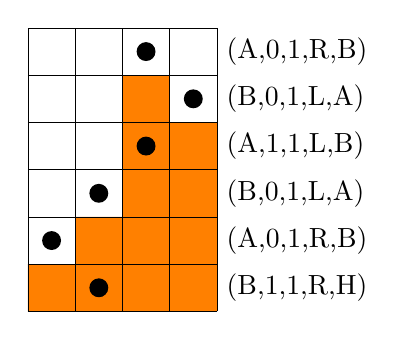
\begin{tikzpicture}[scale=0.6]
                \fill (2.5,-0.5) circle[radius=0.2];
                \draw (4,-0.5)node[right]{(A,0,1,R,B)};
                \fill[orange] (2,-1) rectangle +(1,-1) ;
                \fill (3.5,-1.5) circle[radius=0.2];
                \draw (4,-1.5)node[right]{(B,0,1,L,A)};
                \fill[orange] (2,-2) rectangle +(1,-1) (3,-2) rectangle +(1,-1) ;
                \fill (2.5,-2.5) circle[radius=0.2];
                \draw (4,-2.5)node[right]{(A,1,1,L,B)};
                \fill[orange] (2,-3) rectangle +(1,-1) (3,-3) rectangle +(1,-1) ;
                \fill (1.5,-3.5) circle[radius=0.2];
                \draw (4,-3.5)node[right]{(B,0,1,L,A)};
                \fill[orange] (1,-4) rectangle +(1,-1) (2,-4) rectangle +(1,-1) (3,-4) rectangle +(1,-1) ;
                \fill (0.5,-4.5) circle[radius=0.2];
                \draw (4,-4.5)node[right]{(A,0,1,R,B)};
                \fill[orange] (0,-5) rectangle +(1,-1) (1,-5) rectangle +(1,-1) (2,-5) rectangle +(1,-1) (3,-5) rectangle +(1,-1) ;
                \fill (1.5,-5.5) circle[radius=0.2];
                \draw (4,-5.5)node[right]{(B,1,1,R,H)};
                \draw[help lines, step=1cm, black] (0,0) grid (4,-6);
            \end{tikzpicture}
        \end{center}
    \end{minipage}
    \begin{minipage}{0.45\textwidth}
        \begin{center}
            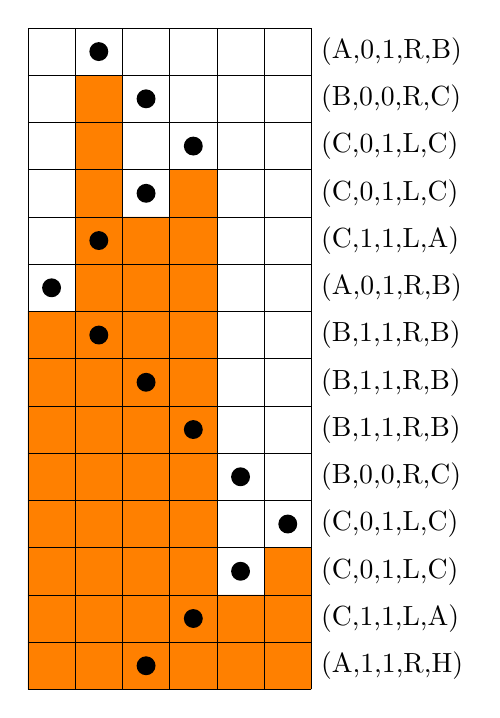
\begin{tikzpicture}[scale=0.6]
                \fill (1.5,-0.5) circle[radius=0.2];
                \draw (6,-0.5)node[right]{(A,0,1,R,B)};
                \fill[orange] (1,-1) rectangle +(1,-1) ;
                \fill (2.5,-1.5) circle[radius=0.2];
                \draw (6,-1.5)node[right]{(B,0,0,R,C)};
                \fill[orange] (1,-2) rectangle +(1,-1) ;
                \fill (3.5,-2.5) circle[radius=0.2];
                \draw (6,-2.5)node[right]{(C,0,1,L,C)};
                \fill[orange] (1,-3) rectangle +(1,-1) (3,-3) rectangle +(1,-1) ;
                \fill (2.5,-3.5) circle[radius=0.2];
                \draw (6,-3.5)node[right]{(C,0,1,L,C)};
                \fill[orange] (1,-4) rectangle +(1,-1) (2,-4) rectangle +(1,-1) (3,-4) rectangle +(1,-1) ;
                \fill (1.5,-4.5) circle[radius=0.2];
                \draw (6,-4.5)node[right]{(C,1,1,L,A)};
                \fill[orange] (1,-5) rectangle +(1,-1) (2,-5) rectangle +(1,-1) (3,-5) rectangle +(1,-1) ;
                \fill (0.5,-5.5) circle[radius=0.2];
                \draw (6,-5.5)node[right]{(A,0,1,R,B)};
                \fill[orange] (0,-6) rectangle +(1,-1) (1,-6) rectangle +(1,-1) (2,-6) rectangle +(1,-1) (3,-6) rectangle +(1,-1) ;
                \fill (1.5,-6.5) circle[radius=0.2];
                \draw (6,-6.5)node[right]{(B,1,1,R,B)};
                \fill[orange] (0,-7) rectangle +(1,-1) (1,-7) rectangle +(1,-1) (2,-7) rectangle +(1,-1) (3,-7) rectangle +(1,-1) ;
                \fill (2.5,-7.5) circle[radius=0.2];
                \draw (6,-7.5)node[right]{(B,1,1,R,B)};
                \fill[orange] (0,-8) rectangle +(1,-1) (1,-8) rectangle +(1,-1) (2,-8) rectangle +(1,-1) (3,-8) rectangle +(1,-1) ;
                \fill (3.5,-8.5) circle[radius=0.2];
                \draw (6,-8.5)node[right]{(B,1,1,R,B)};
                \fill[orange] (0,-9) rectangle +(1,-1) (1,-9) rectangle +(1,-1) (2,-9) rectangle +(1,-1) (3,-9) rectangle +(1,-1) ;
                \fill (4.5,-9.5) circle[radius=0.2];
                \draw (6,-9.5)node[right]{(B,0,0,R,C)};
                \fill[orange] (0,-10) rectangle +(1,-1) (1,-10) rectangle +(1,-1) (2,-10) rectangle +(1,-1) (3,-10) rectangle +(1,-1) ;
                \fill (5.5,-10.5) circle[radius=0.2];
                \draw (6,-10.5)node[right]{(C,0,1,L,C)};
                \fill[orange] (0,-11) rectangle +(1,-1) (1,-11) rectangle +(1,-1) (2,-11) rectangle +(1,-1) (3,-11) rectangle +(1,-1) (5,-11) rectangle +(1,-1) ;
                \fill (4.5,-11.5) circle[radius=0.2];
                \draw (6,-11.5)node[right]{(C,0,1,L,C)};
                \fill[orange] (0,-12) rectangle +(1,-1) (1,-12) rectangle +(1,-1) (2,-12) rectangle +(1,-1) (3,-12) rectangle +(1,-1) (4,-12) rectangle +(1,-1) (5,-12) rectangle +(1,-1) ;
                \fill (3.5,-12.5) circle[radius=0.2];
                \draw (6,-12.5)node[right]{(C,1,1,L,A)};
                \fill[orange] (0,-13) rectangle +(1,-1) (1,-13) rectangle +(1,-1) (2,-13) rectangle +(1,-1) (3,-13) rectangle +(1,-1) (4,-13) rectangle +(1,-1) (5,-13) rectangle +(1,-1) ;
                \fill (2.5,-13.5) circle[radius=0.2];
                \draw (6,-13.5)node[right]{(A,1,1,R,H)};
                \draw[help lines, step=1cm, black] (0,0) grid (6,-14);
            \end{tikzpicture}
        \end{center}
    \end{minipage}
\end{center}

由此可得\(\Sigma(2) = 4\)，\(\Sigma(3) = 6\).

算出\(\Sigma(4)\)的程序如下
\begin{center}
    \begin{tblr}{hlines, vlines, row{1} = {gray9}, column{1} = {gray9}, cells={c}}
        & A & B & C & D \\
      0 & 1RB & 0LA & 1RH & 1RD \\
      1 & 1LB & 0LC & 1LD & 0RA \\
  \end{tblr} 
\end{center}
只有8条指令，却要108步才能停机（图中没有最后一步），其中有一条只能执行一次，剩下都是7条指令来来回回执行.

\begin{multicols}{2}
\begin{center}
    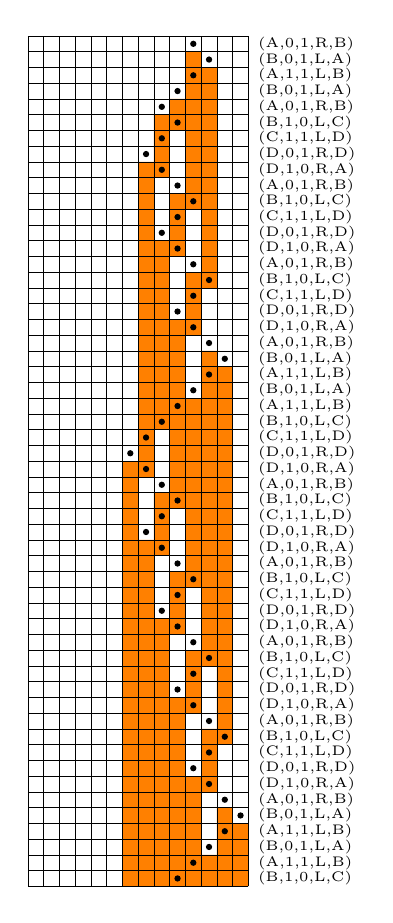
\begin{tikzpicture}[scale=0.2]
        \fill (10.5,-0.5) circle[radius=0.2];
        \draw (14,-0.5)node[right]{\tiny (A,0,1,R,B)};
        \fill[orange] (10,-1) rectangle +(1,-1) ;
        \fill (11.5,-1.5) circle[radius=0.2];
        \draw (14,-1.5)node[right]{\tiny (B,0,1,L,A)};
        \fill[orange] (10,-2) rectangle +(1,-1) (11,-2) rectangle +(1,-1) ;
        \fill (10.5,-2.5) circle[radius=0.2];
        \draw (14,-2.5)node[right]{\tiny (A,1,1,L,B)};
        \fill[orange] (10,-3) rectangle +(1,-1) (11,-3) rectangle +(1,-1) ;
        \fill (9.5,-3.5) circle[radius=0.2];
        \draw (14,-3.5)node[right]{\tiny (B,0,1,L,A)};
        \fill[orange] (9,-4) rectangle +(1,-1) (10,-4) rectangle +(1,-1) (11,-4) rectangle +(1,-1) ;
        \fill (8.5,-4.5) circle[radius=0.2];
        \draw (14,-4.5)node[right]{\tiny (A,0,1,R,B)};
        \fill[orange] (8,-5) rectangle +(1,-1) (9,-5) rectangle +(1,-1) (10,-5) rectangle +(1,-1) (11,-5) rectangle +(1,-1) ;
        \fill (9.5,-5.5) circle[radius=0.2];
        \draw (14,-5.5)node[right]{\tiny (B,1,0,L,C)};
        \fill[orange] (8,-6) rectangle +(1,-1) (10,-6) rectangle +(1,-1) (11,-6) rectangle +(1,-1) ;
        \fill (8.5,-6.5) circle[radius=0.2];
        \draw (14,-6.5)node[right]{\tiny (C,1,1,L,D)};
        \fill[orange] (8,-7) rectangle +(1,-1) (10,-7) rectangle +(1,-1) (11,-7) rectangle +(1,-1) ;
        \fill (7.5,-7.5) circle[radius=0.2];
        \draw (14,-7.5)node[right]{\tiny (D,0,1,R,D)};
        \fill[orange] (7,-8) rectangle +(1,-1) (8,-8) rectangle +(1,-1) (10,-8) rectangle +(1,-1) (11,-8) rectangle +(1,-1) ;
        \fill (8.5,-8.5) circle[radius=0.2];
        \draw (14,-8.5)node[right]{\tiny (D,1,0,R,A)};
        \fill[orange] (7,-9) rectangle +(1,-1) (10,-9) rectangle +(1,-1) (11,-9) rectangle +(1,-1) ;
        \fill (9.5,-9.5) circle[radius=0.2];
        \draw (14,-9.5)node[right]{\tiny (A,0,1,R,B)};
        \fill[orange] (7,-10) rectangle +(1,-1) (9,-10) rectangle +(1,-1) (10,-10) rectangle +(1,-1) (11,-10) rectangle +(1,-1) ;
        \fill (10.5,-10.5) circle[radius=0.2];
        \draw (14,-10.5)node[right]{\tiny (B,1,0,L,C)};
        \fill[orange] (7,-11) rectangle +(1,-1) (9,-11) rectangle +(1,-1) (11,-11) rectangle +(1,-1) ;
        \fill (9.5,-11.5) circle[radius=0.2];
        \draw (14,-11.5)node[right]{\tiny (C,1,1,L,D)};
        \fill[orange] (7,-12) rectangle +(1,-1) (9,-12) rectangle +(1,-1) (11,-12) rectangle +(1,-1) ;
        \fill (8.5,-12.5) circle[radius=0.2];
        \draw (14,-12.5)node[right]{\tiny (D,0,1,R,D)};
        \fill[orange] (7,-13) rectangle +(1,-1) (8,-13) rectangle +(1,-1) (9,-13) rectangle +(1,-1) (11,-13) rectangle +(1,-1) ;
        \fill (9.5,-13.5) circle[radius=0.2];
        \draw (14,-13.5)node[right]{\tiny (D,1,0,R,A)};
        \fill[orange] (7,-14) rectangle +(1,-1) (8,-14) rectangle +(1,-1) (11,-14) rectangle +(1,-1) ;
        \fill (10.5,-14.5) circle[radius=0.2];
        \draw (14,-14.5)node[right]{\tiny (A,0,1,R,B)};
        \fill[orange] (7,-15) rectangle +(1,-1) (8,-15) rectangle +(1,-1) (10,-15) rectangle +(1,-1) (11,-15) rectangle +(1,-1) ;
        \fill (11.5,-15.5) circle[radius=0.2];
        \draw (14,-15.5)node[right]{\tiny (B,1,0,L,C)};
        \fill[orange] (7,-16) rectangle +(1,-1) (8,-16) rectangle +(1,-1) (10,-16) rectangle +(1,-1) ;
        \fill (10.5,-16.5) circle[radius=0.2];
        \draw (14,-16.5)node[right]{\tiny (C,1,1,L,D)};
        \fill[orange] (7,-17) rectangle +(1,-1) (8,-17) rectangle +(1,-1) (10,-17) rectangle +(1,-1) ;
        \fill (9.5,-17.5) circle[radius=0.2];
        \draw (14,-17.5)node[right]{\tiny (D,0,1,R,D)};
        \fill[orange] (7,-18) rectangle +(1,-1) (8,-18) rectangle +(1,-1) (9,-18) rectangle +(1,-1) (10,-18) rectangle +(1,-1) ;
        \fill (10.5,-18.5) circle[radius=0.2];
        \draw (14,-18.5)node[right]{\tiny (D,1,0,R,A)};
        \fill[orange] (7,-19) rectangle +(1,-1) (8,-19) rectangle +(1,-1) (9,-19) rectangle +(1,-1) ;
        \fill (11.5,-19.5) circle[radius=0.2];
        \draw (14,-19.5)node[right]{\tiny (A,0,1,R,B)};
        \fill[orange] (7,-20) rectangle +(1,-1) (8,-20) rectangle +(1,-1) (9,-20) rectangle +(1,-1) (11,-20) rectangle +(1,-1) ;
        \fill (12.5,-20.5) circle[radius=0.2];
        \draw (14,-20.5)node[right]{\tiny (B,0,1,L,A)};
        \fill[orange] (7,-21) rectangle +(1,-1) (8,-21) rectangle +(1,-1) (9,-21) rectangle +(1,-1) (11,-21) rectangle +(1,-1) (12,-21) rectangle +(1,-1) ;
        \fill (11.5,-21.5) circle[radius=0.2];
        \draw (14,-21.5)node[right]{\tiny (A,1,1,L,B)};
        \fill[orange] (7,-22) rectangle +(1,-1) (8,-22) rectangle +(1,-1) (9,-22) rectangle +(1,-1) (11,-22) rectangle +(1,-1) (12,-22) rectangle +(1,-1) ;
        \fill (10.5,-22.5) circle[radius=0.2];
        \draw (14,-22.5)node[right]{\tiny (B,0,1,L,A)};
        \fill[orange] (7,-23) rectangle +(1,-1) (8,-23) rectangle +(1,-1) (9,-23) rectangle +(1,-1) (10,-23) rectangle +(1,-1) (11,-23) rectangle +(1,-1) (12,-23) rectangle +(1,-1) ;
        \fill (9.5,-23.5) circle[radius=0.2];
        \draw (14,-23.5)node[right]{\tiny (A,1,1,L,B)};
        \fill[orange] (7,-24) rectangle +(1,-1) (8,-24) rectangle +(1,-1) (9,-24) rectangle +(1,-1) (10,-24) rectangle +(1,-1) (11,-24) rectangle +(1,-1) (12,-24) rectangle +(1,-1) ;
        \fill (8.5,-24.5) circle[radius=0.2];
        \draw (14,-24.5)node[right]{\tiny (B,1,0,L,C)};
        \fill[orange] (7,-25) rectangle +(1,-1) (9,-25) rectangle +(1,-1) (10,-25) rectangle +(1,-1) (11,-25) rectangle +(1,-1) (12,-25) rectangle +(1,-1) ;
        \fill (7.5,-25.5) circle[radius=0.2];
        \draw (14,-25.5)node[right]{\tiny (C,1,1,L,D)};
        \fill[orange] (7,-26) rectangle +(1,-1) (9,-26) rectangle +(1,-1) (10,-26) rectangle +(1,-1) (11,-26) rectangle +(1,-1) (12,-26) rectangle +(1,-1) ;
        \fill (6.5,-26.5) circle[radius=0.2];
        \draw (14,-26.5)node[right]{\tiny (D,0,1,R,D)};
        \fill[orange] (6,-27) rectangle +(1,-1) (7,-27) rectangle +(1,-1) (9,-27) rectangle +(1,-1) (10,-27) rectangle +(1,-1) (11,-27) rectangle +(1,-1) (12,-27) rectangle +(1,-1) ;
        \fill (7.5,-27.5) circle[radius=0.2];
        \draw (14,-27.5)node[right]{\tiny (D,1,0,R,A)};
        \fill[orange] (6,-28) rectangle +(1,-1) (9,-28) rectangle +(1,-1) (10,-28) rectangle +(1,-1) (11,-28) rectangle +(1,-1) (12,-28) rectangle +(1,-1) ;
        \fill (8.5,-28.5) circle[radius=0.2];
        \draw (14,-28.5)node[right]{\tiny (A,0,1,R,B)};
        \fill[orange] (6,-29) rectangle +(1,-1) (8,-29) rectangle +(1,-1) (9,-29) rectangle +(1,-1) (10,-29) rectangle +(1,-1) (11,-29) rectangle +(1,-1) (12,-29) rectangle +(1,-1) ;
        \fill (9.5,-29.5) circle[radius=0.2];
        \draw (14,-29.5)node[right]{\tiny (B,1,0,L,C)};
        \fill[orange] (6,-30) rectangle +(1,-1) (8,-30) rectangle +(1,-1) (10,-30) rectangle +(1,-1) (11,-30) rectangle +(1,-1) (12,-30) rectangle +(1,-1) ;
        \fill (8.5,-30.5) circle[radius=0.2];
        \draw (14,-30.5)node[right]{\tiny (C,1,1,L,D)};
        \fill[orange] (6,-31) rectangle +(1,-1) (8,-31) rectangle +(1,-1) (10,-31) rectangle +(1,-1) (11,-31) rectangle +(1,-1) (12,-31) rectangle +(1,-1) ;
        \fill (7.5,-31.5) circle[radius=0.2];
        \draw (14,-31.5)node[right]{\tiny (D,0,1,R,D)};
        \fill[orange] (6,-32) rectangle +(1,-1) (7,-32) rectangle +(1,-1) (8,-32) rectangle +(1,-1) (10,-32) rectangle +(1,-1) (11,-32) rectangle +(1,-1) (12,-32) rectangle +(1,-1) ;
        \fill (8.5,-32.5) circle[radius=0.2];
        \draw (14,-32.5)node[right]{\tiny (D,1,0,R,A)};
        \fill[orange] (6,-33) rectangle +(1,-1) (7,-33) rectangle +(1,-1) (10,-33) rectangle +(1,-1) (11,-33) rectangle +(1,-1) (12,-33) rectangle +(1,-1) ;
        \fill (9.5,-33.5) circle[radius=0.2];
        \draw (14,-33.5)node[right]{\tiny (A,0,1,R,B)};
        \fill[orange] (6,-34) rectangle +(1,-1) (7,-34) rectangle +(1,-1) (9,-34) rectangle +(1,-1) (10,-34) rectangle +(1,-1) (11,-34) rectangle +(1,-1) (12,-34) rectangle +(1,-1) ;
        \fill (10.5,-34.5) circle[radius=0.2];
        \draw (14,-34.5)node[right]{\tiny (B,1,0,L,C)};
        \fill[orange] (6,-35) rectangle +(1,-1) (7,-35) rectangle +(1,-1) (9,-35) rectangle +(1,-1) (11,-35) rectangle +(1,-1) (12,-35) rectangle +(1,-1) ;
        \fill (9.5,-35.5) circle[radius=0.2];
        \draw (14,-35.5)node[right]{\tiny (C,1,1,L,D)};
        \fill[orange] (6,-36) rectangle +(1,-1) (7,-36) rectangle +(1,-1) (9,-36) rectangle +(1,-1) (11,-36) rectangle +(1,-1) (12,-36) rectangle +(1,-1) ;
        \fill (8.5,-36.5) circle[radius=0.2];
        \draw (14,-36.5)node[right]{\tiny (D,0,1,R,D)};
        \fill[orange] (6,-37) rectangle +(1,-1) (7,-37) rectangle +(1,-1) (8,-37) rectangle +(1,-1) (9,-37) rectangle +(1,-1) (11,-37) rectangle +(1,-1) (12,-37) rectangle +(1,-1) ;
        \fill (9.5,-37.5) circle[radius=0.2];
        \draw (14,-37.5)node[right]{\tiny (D,1,0,R,A)};
        \fill[orange] (6,-38) rectangle +(1,-1) (7,-38) rectangle +(1,-1) (8,-38) rectangle +(1,-1) (11,-38) rectangle +(1,-1) (12,-38) rectangle +(1,-1) ;
        \fill (10.5,-38.5) circle[radius=0.2];
        \draw (14,-38.5)node[right]{\tiny (A,0,1,R,B)};
        \fill[orange] (6,-39) rectangle +(1,-1) (7,-39) rectangle +(1,-1) (8,-39) rectangle +(1,-1) (10,-39) rectangle +(1,-1) (11,-39) rectangle +(1,-1) (12,-39) rectangle +(1,-1) ;
        \fill (11.5,-39.5) circle[radius=0.2];
        \draw (14,-39.5)node[right]{\tiny (B,1,0,L,C)};
        \fill[orange] (6,-40) rectangle +(1,-1) (7,-40) rectangle +(1,-1) (8,-40) rectangle +(1,-1) (10,-40) rectangle +(1,-1) (12,-40) rectangle +(1,-1) ;
        \fill (10.5,-40.5) circle[radius=0.2];
        \draw (14,-40.5)node[right]{\tiny (C,1,1,L,D)};
        \fill[orange] (6,-41) rectangle +(1,-1) (7,-41) rectangle +(1,-1) (8,-41) rectangle +(1,-1) (10,-41) rectangle +(1,-1) (12,-41) rectangle +(1,-1) ;
        \fill (9.5,-41.5) circle[radius=0.2];
        \draw (14,-41.5)node[right]{\tiny (D,0,1,R,D)};
        \fill[orange] (6,-42) rectangle +(1,-1) (7,-42) rectangle +(1,-1) (8,-42) rectangle +(1,-1) (9,-42) rectangle +(1,-1) (10,-42) rectangle +(1,-1) (12,-42) rectangle +(1,-1) ;
        \fill (10.5,-42.5) circle[radius=0.2];
        \draw (14,-42.5)node[right]{\tiny (D,1,0,R,A)};
        \fill[orange] (6,-43) rectangle +(1,-1) (7,-43) rectangle +(1,-1) (8,-43) rectangle +(1,-1) (9,-43) rectangle +(1,-1) (12,-43) rectangle +(1,-1) ;
        \fill (11.5,-43.5) circle[radius=0.2];
        \draw (14,-43.5)node[right]{\tiny (A,0,1,R,B)};
        \fill[orange] (6,-44) rectangle +(1,-1) (7,-44) rectangle +(1,-1) (8,-44) rectangle +(1,-1) (9,-44) rectangle +(1,-1) (11,-44) rectangle +(1,-1) (12,-44) rectangle +(1,-1) ;
        \fill (12.5,-44.5) circle[radius=0.2];
        \draw (14,-44.5)node[right]{\tiny (B,1,0,L,C)};
        \fill[orange] (6,-45) rectangle +(1,-1) (7,-45) rectangle +(1,-1) (8,-45) rectangle +(1,-1) (9,-45) rectangle +(1,-1) (11,-45) rectangle +(1,-1) ;
        \fill (11.5,-45.5) circle[radius=0.2];
        \draw (14,-45.5)node[right]{\tiny (C,1,1,L,D)};
        \fill[orange] (6,-46) rectangle +(1,-1) (7,-46) rectangle +(1,-1) (8,-46) rectangle +(1,-1) (9,-46) rectangle +(1,-1) (11,-46) rectangle +(1,-1) ;
        \fill (10.5,-46.5) circle[radius=0.2];
        \draw (14,-46.5)node[right]{\tiny (D,0,1,R,D)};
        \fill[orange] (6,-47) rectangle +(1,-1) (7,-47) rectangle +(1,-1) (8,-47) rectangle +(1,-1) (9,-47) rectangle +(1,-1) (10,-47) rectangle +(1,-1) (11,-47) rectangle +(1,-1) ;
        \fill (11.5,-47.5) circle[radius=0.2];
        \draw (14,-47.5)node[right]{\tiny (D,1,0,R,A)};
        \fill[orange] (6,-48) rectangle +(1,-1) (7,-48) rectangle +(1,-1) (8,-48) rectangle +(1,-1) (9,-48) rectangle +(1,-1) (10,-48) rectangle +(1,-1) ;
        \fill (12.5,-48.5) circle[radius=0.2];
        \draw (14,-48.5)node[right]{\tiny (A,0,1,R,B)};
        \fill[orange] (6,-49) rectangle +(1,-1) (7,-49) rectangle +(1,-1) (8,-49) rectangle +(1,-1) (9,-49) rectangle +(1,-1) (10,-49) rectangle +(1,-1) (12,-49) rectangle +(1,-1) ;
        \fill (13.5,-49.5) circle[radius=0.2];
        \draw (14,-49.5)node[right]{\tiny (B,0,1,L,A)};
        \fill[orange] (6,-50) rectangle +(1,-1) (7,-50) rectangle +(1,-1) (8,-50) rectangle +(1,-1) (9,-50) rectangle +(1,-1) (10,-50) rectangle +(1,-1) (12,-50) rectangle +(1,-1) (13,-50) rectangle +(1,-1) ;
        \fill (12.5,-50.5) circle[radius=0.2];
        \draw (14,-50.5)node[right]{\tiny (A,1,1,L,B)};
        \fill[orange] (6,-51) rectangle +(1,-1) (7,-51) rectangle +(1,-1) (8,-51) rectangle +(1,-1) (9,-51) rectangle +(1,-1) (10,-51) rectangle +(1,-1) (12,-51) rectangle +(1,-1) (13,-51) rectangle +(1,-1) ;
        \fill (11.5,-51.5) circle[radius=0.2];
        \draw (14,-51.5)node[right]{\tiny (B,0,1,L,A)};
        \fill[orange] (6,-52) rectangle +(1,-1) (7,-52) rectangle +(1,-1) (8,-52) rectangle +(1,-1) (9,-52) rectangle +(1,-1) (10,-52) rectangle +(1,-1) (11,-52) rectangle +(1,-1) (12,-52) rectangle +(1,-1) (13,-52) rectangle +(1,-1) ;
        \fill (10.5,-52.5) circle[radius=0.2];
        \draw (14,-52.5)node[right]{\tiny (A,1,1,L,B)};
        \fill[orange] (6,-53) rectangle +(1,-1) (7,-53) rectangle +(1,-1) (8,-53) rectangle +(1,-1) (9,-53) rectangle +(1,-1) (10,-53) rectangle +(1,-1) (11,-53) rectangle +(1,-1) (12,-53) rectangle +(1,-1) (13,-53) rectangle +(1,-1) ;
        \fill (9.5,-53.5) circle[radius=0.2];
        \draw (14,-53.5)node[right]{\tiny (B,1,0,L,C)};
        \draw[help lines,step=1cm,black] (0,0) grid (14,-54);
    \end{tikzpicture}
    \end{center}
   
    \begin{center}
    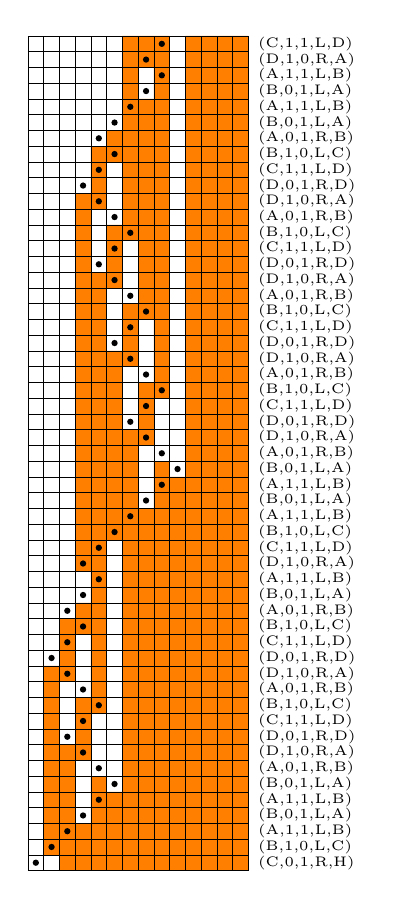
\begin{tikzpicture}[scale=0.2]
        \fill[orange] (6,-54) rectangle +(1,-1) (7,-54) rectangle +(1,-1) (8,-54) rectangle +(1,-1) (10,-54) rectangle +(1,-1) (11,-54) rectangle +(1,-1) (12,-54) rectangle +(1,-1) (13,-54) rectangle +(1,-1) ;
        \fill (8.5,-54.5) circle[radius=0.2];
        \draw (14,-54.5)node[right]{\tiny (C,1,1,L,D)};
        \fill[orange] (6,-55) rectangle +(1,-1) (7,-55) rectangle +(1,-1) (8,-55) rectangle +(1,-1) (10,-55) rectangle +(1,-1) (11,-55) rectangle +(1,-1) (12,-55) rectangle +(1,-1) (13,-55) rectangle +(1,-1) ;
        \fill (7.5,-55.5) circle[radius=0.2];
        \draw (14,-55.5)node[right]{\tiny (D,1,0,R,A)};
        \fill[orange] (6,-56) rectangle +(1,-1) (8,-56) rectangle +(1,-1) (10,-56) rectangle +(1,-1) (11,-56) rectangle +(1,-1) (12,-56) rectangle +(1,-1) (13,-56) rectangle +(1,-1) ;
        \fill (8.5,-56.5) circle[radius=0.2];
        \draw (14,-56.5)node[right]{\tiny (A,1,1,L,B)};
        \fill[orange] (6,-57) rectangle +(1,-1) (8,-57) rectangle +(1,-1) (10,-57) rectangle +(1,-1) (11,-57) rectangle +(1,-1) (12,-57) rectangle +(1,-1) (13,-57) rectangle +(1,-1) ;
        \fill (7.5,-57.5) circle[radius=0.2];
        \draw (14,-57.5)node[right]{\tiny (B,0,1,L,A)};
        \fill[orange] (6,-58) rectangle +(1,-1) (7,-58) rectangle +(1,-1) (8,-58) rectangle +(1,-1) (10,-58) rectangle +(1,-1) (11,-58) rectangle +(1,-1) (12,-58) rectangle +(1,-1) (13,-58) rectangle +(1,-1) ;
        \fill (6.5,-58.5) circle[radius=0.2];
        \draw (14,-58.5)node[right]{\tiny (A,1,1,L,B)};
        \fill[orange] (6,-59) rectangle +(1,-1) (7,-59) rectangle +(1,-1) (8,-59) rectangle +(1,-1) (10,-59) rectangle +(1,-1) (11,-59) rectangle +(1,-1) (12,-59) rectangle +(1,-1) (13,-59) rectangle +(1,-1) ;
        \fill (5.5,-59.5) circle[radius=0.2];
        \draw (14,-59.5)node[right]{\tiny (B,0,1,L,A)};
        \fill[orange] (5,-60) rectangle +(1,-1) (6,-60) rectangle +(1,-1) (7,-60) rectangle +(1,-1) (8,-60) rectangle +(1,-1) (10,-60) rectangle +(1,-1) (11,-60) rectangle +(1,-1) (12,-60) rectangle +(1,-1) (13,-60) rectangle +(1,-1) ;
        \fill (4.5,-60.5) circle[radius=0.2];
        \draw (14,-60.5)node[right]{\tiny (A,0,1,R,B)};
        \fill[orange] (4,-61) rectangle +(1,-1) (5,-61) rectangle +(1,-1) (6,-61) rectangle +(1,-1) (7,-61) rectangle +(1,-1) (8,-61) rectangle +(1,-1) (10,-61) rectangle +(1,-1) (11,-61) rectangle +(1,-1) (12,-61) rectangle +(1,-1) (13,-61) rectangle +(1,-1) ;
        \fill (5.5,-61.5) circle[radius=0.2];
        \draw (14,-61.5)node[right]{\tiny (B,1,0,L,C)};
        \fill[orange] (4,-62) rectangle +(1,-1) (6,-62) rectangle +(1,-1) (7,-62) rectangle +(1,-1) (8,-62) rectangle +(1,-1) (10,-62) rectangle +(1,-1) (11,-62) rectangle +(1,-1) (12,-62) rectangle +(1,-1) (13,-62) rectangle +(1,-1) ;
        \fill (4.5,-62.5) circle[radius=0.2];
        \draw (14,-62.5)node[right]{\tiny (C,1,1,L,D)};
        \fill[orange] (4,-63) rectangle +(1,-1) (6,-63) rectangle +(1,-1) (7,-63) rectangle +(1,-1) (8,-63) rectangle +(1,-1) (10,-63) rectangle +(1,-1) (11,-63) rectangle +(1,-1) (12,-63) rectangle +(1,-1) (13,-63) rectangle +(1,-1) ;
        \fill (3.5,-63.5) circle[radius=0.2];
        \draw (14,-63.5)node[right]{\tiny (D,0,1,R,D)};
        \fill[orange] (3,-64) rectangle +(1,-1) (4,-64) rectangle +(1,-1) (6,-64) rectangle +(1,-1) (7,-64) rectangle +(1,-1) (8,-64) rectangle +(1,-1) (10,-64) rectangle +(1,-1) (11,-64) rectangle +(1,-1) (12,-64) rectangle +(1,-1) (13,-64) rectangle +(1,-1) ;
        \fill (4.5,-64.5) circle[radius=0.2];
        \draw (14,-64.5)node[right]{\tiny (D,1,0,R,A)};
        \fill[orange] (3,-65) rectangle +(1,-1) (6,-65) rectangle +(1,-1) (7,-65) rectangle +(1,-1) (8,-65) rectangle +(1,-1) (10,-65) rectangle +(1,-1) (11,-65) rectangle +(1,-1) (12,-65) rectangle +(1,-1) (13,-65) rectangle +(1,-1) ;
        \fill (5.5,-65.5) circle[radius=0.2];
        \draw (14,-65.5)node[right]{\tiny (A,0,1,R,B)};
        \fill[orange] (3,-66) rectangle +(1,-1) (5,-66) rectangle +(1,-1) (6,-66) rectangle +(1,-1) (7,-66) rectangle +(1,-1) (8,-66) rectangle +(1,-1) (10,-66) rectangle +(1,-1) (11,-66) rectangle +(1,-1) (12,-66) rectangle +(1,-1) (13,-66) rectangle +(1,-1) ;
        \fill (6.5,-66.5) circle[radius=0.2];
        \draw (14,-66.5)node[right]{\tiny (B,1,0,L,C)};
        \fill[orange] (3,-67) rectangle +(1,-1) (5,-67) rectangle +(1,-1) (7,-67) rectangle +(1,-1) (8,-67) rectangle +(1,-1) (10,-67) rectangle +(1,-1) (11,-67) rectangle +(1,-1) (12,-67) rectangle +(1,-1) (13,-67) rectangle +(1,-1) ;
        \fill (5.5,-67.5) circle[radius=0.2];
        \draw (14,-67.5)node[right]{\tiny (C,1,1,L,D)};
        \fill[orange] (3,-68) rectangle +(1,-1) (5,-68) rectangle +(1,-1) (7,-68) rectangle +(1,-1) (8,-68) rectangle +(1,-1) (10,-68) rectangle +(1,-1) (11,-68) rectangle +(1,-1) (12,-68) rectangle +(1,-1) (13,-68) rectangle +(1,-1) ;
        \fill (4.5,-68.5) circle[radius=0.2];
        \draw (14,-68.5)node[right]{\tiny (D,0,1,R,D)};
        \fill[orange] (3,-69) rectangle +(1,-1) (4,-69) rectangle +(1,-1) (5,-69) rectangle +(1,-1) (7,-69) rectangle +(1,-1) (8,-69) rectangle +(1,-1) (10,-69) rectangle +(1,-1) (11,-69) rectangle +(1,-1) (12,-69) rectangle +(1,-1) (13,-69) rectangle +(1,-1) ;
        \fill (5.5,-69.5) circle[radius=0.2];
        \draw (14,-69.5)node[right]{\tiny (D,1,0,R,A)};
        \fill[orange] (3,-70) rectangle +(1,-1) (4,-70) rectangle +(1,-1) (7,-70) rectangle +(1,-1) (8,-70) rectangle +(1,-1) (10,-70) rectangle +(1,-1) (11,-70) rectangle +(1,-1) (12,-70) rectangle +(1,-1) (13,-70) rectangle +(1,-1) ;
        \fill (6.5,-70.5) circle[radius=0.2];
        \draw (14,-70.5)node[right]{\tiny (A,0,1,R,B)};
        \fill[orange] (3,-71) rectangle +(1,-1) (4,-71) rectangle +(1,-1) (6,-71) rectangle +(1,-1) (7,-71) rectangle +(1,-1) (8,-71) rectangle +(1,-1) (10,-71) rectangle +(1,-1) (11,-71) rectangle +(1,-1) (12,-71) rectangle +(1,-1) (13,-71) rectangle +(1,-1) ;
        \fill (7.5,-71.5) circle[radius=0.2];
        \draw (14,-71.5)node[right]{\tiny (B,1,0,L,C)};
        \fill[orange] (3,-72) rectangle +(1,-1) (4,-72) rectangle +(1,-1) (6,-72) rectangle +(1,-1) (8,-72) rectangle +(1,-1) (10,-72) rectangle +(1,-1) (11,-72) rectangle +(1,-1) (12,-72) rectangle +(1,-1) (13,-72) rectangle +(1,-1) ;
        \fill (6.5,-72.5) circle[radius=0.2];
        \draw (14,-72.5)node[right]{\tiny (C,1,1,L,D)};
        \fill[orange] (3,-73) rectangle +(1,-1) (4,-73) rectangle +(1,-1) (6,-73) rectangle +(1,-1) (8,-73) rectangle +(1,-1) (10,-73) rectangle +(1,-1) (11,-73) rectangle +(1,-1) (12,-73) rectangle +(1,-1) (13,-73) rectangle +(1,-1) ;
        \fill (5.5,-73.5) circle[radius=0.2];
        \draw (14,-73.5)node[right]{\tiny (D,0,1,R,D)};
        \fill[orange] (3,-74) rectangle +(1,-1) (4,-74) rectangle +(1,-1) (5,-74) rectangle +(1,-1) (6,-74) rectangle +(1,-1) (8,-74) rectangle +(1,-1) (10,-74) rectangle +(1,-1) (11,-74) rectangle +(1,-1) (12,-74) rectangle +(1,-1) (13,-74) rectangle +(1,-1) ;
        \fill (6.5,-74.5) circle[radius=0.2];
        \draw (14,-74.5)node[right]{\tiny (D,1,0,R,A)};
        \fill[orange] (3,-75) rectangle +(1,-1) (4,-75) rectangle +(1,-1) (5,-75) rectangle +(1,-1) (8,-75) rectangle +(1,-1) (10,-75) rectangle +(1,-1) (11,-75) rectangle +(1,-1) (12,-75) rectangle +(1,-1) (13,-75) rectangle +(1,-1) ;
        \fill (7.5,-75.5) circle[radius=0.2];
        \draw (14,-75.5)node[right]{\tiny (A,0,1,R,B)};
        \fill[orange] (3,-76) rectangle +(1,-1) (4,-76) rectangle +(1,-1) (5,-76) rectangle +(1,-1) (7,-76) rectangle +(1,-1) (8,-76) rectangle +(1,-1) (10,-76) rectangle +(1,-1) (11,-76) rectangle +(1,-1) (12,-76) rectangle +(1,-1) (13,-76) rectangle +(1,-1) ;
        \fill (8.5,-76.5) circle[radius=0.2];
        \draw (14,-76.5)node[right]{\tiny (B,1,0,L,C)};
        \fill[orange] (3,-77) rectangle +(1,-1) (4,-77) rectangle +(1,-1) (5,-77) rectangle +(1,-1) (7,-77) rectangle +(1,-1) (10,-77) rectangle +(1,-1) (11,-77) rectangle +(1,-1) (12,-77) rectangle +(1,-1) (13,-77) rectangle +(1,-1) ;
        \fill (7.5,-77.5) circle[radius=0.2];
        \draw (14,-77.5)node[right]{\tiny (C,1,1,L,D)};
        \fill[orange] (3,-78) rectangle +(1,-1) (4,-78) rectangle +(1,-1) (5,-78) rectangle +(1,-1) (7,-78) rectangle +(1,-1) (10,-78) rectangle +(1,-1) (11,-78) rectangle +(1,-1) (12,-78) rectangle +(1,-1) (13,-78) rectangle +(1,-1) ;
        \fill (6.5,-78.5) circle[radius=0.2];
        \draw (14,-78.5)node[right]{\tiny (D,0,1,R,D)};
        \fill[orange] (3,-79) rectangle +(1,-1) (4,-79) rectangle +(1,-1) (5,-79) rectangle +(1,-1) (6,-79) rectangle +(1,-1) (7,-79) rectangle +(1,-1) (10,-79) rectangle +(1,-1) (11,-79) rectangle +(1,-1) (12,-79) rectangle +(1,-1) (13,-79) rectangle +(1,-1) ;
        \fill (7.5,-79.5) circle[radius=0.2];
        \draw (14,-79.5)node[right]{\tiny (D,1,0,R,A)};
        \fill[orange] (3,-80) rectangle +(1,-1) (4,-80) rectangle +(1,-1) (5,-80) rectangle +(1,-1) (6,-80) rectangle +(1,-1) (10,-80) rectangle +(1,-1) (11,-80) rectangle +(1,-1) (12,-80) rectangle +(1,-1) (13,-80) rectangle +(1,-1) ;
        \fill (8.5,-80.5) circle[radius=0.2];
        \draw (14,-80.5)node[right]{\tiny (A,0,1,R,B)};
        \fill[orange] (3,-81) rectangle +(1,-1) (4,-81) rectangle +(1,-1) (5,-81) rectangle +(1,-1) (6,-81) rectangle +(1,-1) (8,-81) rectangle +(1,-1) (10,-81) rectangle +(1,-1) (11,-81) rectangle +(1,-1) (12,-81) rectangle +(1,-1) (13,-81) rectangle +(1,-1) ;
        \fill (9.5,-81.5) circle[radius=0.2];
        \draw (14,-81.5)node[right]{\tiny (B,0,1,L,A)};
        \fill[orange] (3,-82) rectangle +(1,-1) (4,-82) rectangle +(1,-1) (5,-82) rectangle +(1,-1) (6,-82) rectangle +(1,-1) (8,-82) rectangle +(1,-1) (9,-82) rectangle +(1,-1) (10,-82) rectangle +(1,-1) (11,-82) rectangle +(1,-1) (12,-82) rectangle +(1,-1) (13,-82) rectangle +(1,-1) ;
        \fill (8.5,-82.5) circle[radius=0.2];
        \draw (14,-82.5)node[right]{\tiny (A,1,1,L,B)};
        \fill[orange] (3,-83) rectangle +(1,-1) (4,-83) rectangle +(1,-1) (5,-83) rectangle +(1,-1) (6,-83) rectangle +(1,-1) (8,-83) rectangle +(1,-1) (9,-83) rectangle +(1,-1) (10,-83) rectangle +(1,-1) (11,-83) rectangle +(1,-1) (12,-83) rectangle +(1,-1) (13,-83) rectangle +(1,-1) ;
        \fill (7.5,-83.5) circle[radius=0.2];
        \draw (14,-83.5)node[right]{\tiny (B,0,1,L,A)};
        \fill[orange] (3,-84) rectangle +(1,-1) (4,-84) rectangle +(1,-1) (5,-84) rectangle +(1,-1) (6,-84) rectangle +(1,-1) (7,-84) rectangle +(1,-1) (8,-84) rectangle +(1,-1) (9,-84) rectangle +(1,-1) (10,-84) rectangle +(1,-1) (11,-84) rectangle +(1,-1) (12,-84) rectangle +(1,-1) (13,-84) rectangle +(1,-1) ;
        \fill (6.5,-84.5) circle[radius=0.2];
        \draw (14,-84.5)node[right]{\tiny (A,1,1,L,B)};
        \fill[orange] (3,-85) rectangle +(1,-1) (4,-85) rectangle +(1,-1) (5,-85) rectangle +(1,-1) (6,-85) rectangle +(1,-1) (7,-85) rectangle +(1,-1) (8,-85) rectangle +(1,-1) (9,-85) rectangle +(1,-1) (10,-85) rectangle +(1,-1) (11,-85) rectangle +(1,-1) (12,-85) rectangle +(1,-1) (13,-85) rectangle +(1,-1) ;
        \fill (5.5,-85.5) circle[radius=0.2];
        \draw (14,-85.5)node[right]{\tiny (B,1,0,L,C)};
        \fill[orange] (3,-86) rectangle +(1,-1) (4,-86) rectangle +(1,-1) (6,-86) rectangle +(1,-1) (7,-86) rectangle +(1,-1) (8,-86) rectangle +(1,-1) (9,-86) rectangle +(1,-1) (10,-86) rectangle +(1,-1) (11,-86) rectangle +(1,-1) (12,-86) rectangle +(1,-1) (13,-86) rectangle +(1,-1) ;
        \fill (4.5,-86.5) circle[radius=0.2];
        \draw (14,-86.5)node[right]{\tiny (C,1,1,L,D)};
        \fill[orange] (3,-87) rectangle +(1,-1) (4,-87) rectangle +(1,-1) (6,-87) rectangle +(1,-1) (7,-87) rectangle +(1,-1) (8,-87) rectangle +(1,-1) (9,-87) rectangle +(1,-1) (10,-87) rectangle +(1,-1) (11,-87) rectangle +(1,-1) (12,-87) rectangle +(1,-1) (13,-87) rectangle +(1,-1) ;
        \fill (3.5,-87.5) circle[radius=0.2];
        \draw (14,-87.5)node[right]{\tiny (D,1,0,R,A)};
        \fill[orange] (4,-88) rectangle +(1,-1) (6,-88) rectangle +(1,-1) (7,-88) rectangle +(1,-1) (8,-88) rectangle +(1,-1) (9,-88) rectangle +(1,-1) (10,-88) rectangle +(1,-1) (11,-88) rectangle +(1,-1) (12,-88) rectangle +(1,-1) (13,-88) rectangle +(1,-1) ;
        \fill (4.5,-88.5) circle[radius=0.2];
        \draw (14,-88.5)node[right]{\tiny (A,1,1,L,B)};
        \fill[orange] (4,-89) rectangle +(1,-1) (6,-89) rectangle +(1,-1) (7,-89) rectangle +(1,-1) (8,-89) rectangle +(1,-1) (9,-89) rectangle +(1,-1) (10,-89) rectangle +(1,-1) (11,-89) rectangle +(1,-1) (12,-89) rectangle +(1,-1) (13,-89) rectangle +(1,-1) ;
        \fill (3.5,-89.5) circle[radius=0.2];
        \draw (14,-89.5)node[right]{\tiny (B,0,1,L,A)};
        \fill[orange] (3,-90) rectangle +(1,-1) (4,-90) rectangle +(1,-1) (6,-90) rectangle +(1,-1) (7,-90) rectangle +(1,-1) (8,-90) rectangle +(1,-1) (9,-90) rectangle +(1,-1) (10,-90) rectangle +(1,-1) (11,-90) rectangle +(1,-1) (12,-90) rectangle +(1,-1) (13,-90) rectangle +(1,-1) ;
        \fill (2.5,-90.5) circle[radius=0.2];
        \draw (14,-90.5)node[right]{\tiny (A,0,1,R,B)};
        \fill[orange] (2,-91) rectangle +(1,-1) (3,-91) rectangle +(1,-1) (4,-91) rectangle +(1,-1) (6,-91) rectangle +(1,-1) (7,-91) rectangle +(1,-1) (8,-91) rectangle +(1,-1) (9,-91) rectangle +(1,-1) (10,-91) rectangle +(1,-1) (11,-91) rectangle +(1,-1) (12,-91) rectangle +(1,-1) (13,-91) rectangle +(1,-1) ;
        \fill (3.5,-91.5) circle[radius=0.2];
        \draw (14,-91.5)node[right]{\tiny (B,1,0,L,C)};
        \fill[orange] (2,-92) rectangle +(1,-1) (4,-92) rectangle +(1,-1) (6,-92) rectangle +(1,-1) (7,-92) rectangle +(1,-1) (8,-92) rectangle +(1,-1) (9,-92) rectangle +(1,-1) (10,-92) rectangle +(1,-1) (11,-92) rectangle +(1,-1) (12,-92) rectangle +(1,-1) (13,-92) rectangle +(1,-1) ;
        \fill (2.5,-92.5) circle[radius=0.2];
        \draw (14,-92.5)node[right]{\tiny (C,1,1,L,D)};
        \fill[orange] (2,-93) rectangle +(1,-1) (4,-93) rectangle +(1,-1) (6,-93) rectangle +(1,-1) (7,-93) rectangle +(1,-1) (8,-93) rectangle +(1,-1) (9,-93) rectangle +(1,-1) (10,-93) rectangle +(1,-1) (11,-93) rectangle +(1,-1) (12,-93) rectangle +(1,-1) (13,-93) rectangle +(1,-1) ;
        \fill (1.5,-93.5) circle[radius=0.2];
        \draw (14,-93.5)node[right]{\tiny (D,0,1,R,D)};
        \fill[orange] (1,-94) rectangle +(1,-1) (2,-94) rectangle +(1,-1) (4,-94) rectangle +(1,-1) (6,-94) rectangle +(1,-1) (7,-94) rectangle +(1,-1) (8,-94) rectangle +(1,-1) (9,-94) rectangle +(1,-1) (10,-94) rectangle +(1,-1) (11,-94) rectangle +(1,-1) (12,-94) rectangle +(1,-1) (13,-94) rectangle +(1,-1) ;
        \fill (2.5,-94.5) circle[radius=0.2];
        \draw (14,-94.5)node[right]{\tiny (D,1,0,R,A)};
        \fill[orange] (1,-95) rectangle +(1,-1) (4,-95) rectangle +(1,-1) (6,-95) rectangle +(1,-1) (7,-95) rectangle +(1,-1) (8,-95) rectangle +(1,-1) (9,-95) rectangle +(1,-1) (10,-95) rectangle +(1,-1) (11,-95) rectangle +(1,-1) (12,-95) rectangle +(1,-1) (13,-95) rectangle +(1,-1) ;
        \fill (3.5,-95.5) circle[radius=0.2];
        \draw (14,-95.5)node[right]{\tiny (A,0,1,R,B)};
        \fill[orange] (1,-96) rectangle +(1,-1) (3,-96) rectangle +(1,-1) (4,-96) rectangle +(1,-1) (6,-96) rectangle +(1,-1) (7,-96) rectangle +(1,-1) (8,-96) rectangle +(1,-1) (9,-96) rectangle +(1,-1) (10,-96) rectangle +(1,-1) (11,-96) rectangle +(1,-1) (12,-96) rectangle +(1,-1) (13,-96) rectangle +(1,-1) ;
        \fill (4.5,-96.5) circle[radius=0.2];
        \draw (14,-96.5)node[right]{\tiny (B,1,0,L,C)};
        \fill[orange] (1,-97) rectangle +(1,-1) (3,-97) rectangle +(1,-1) (6,-97) rectangle +(1,-1) (7,-97) rectangle +(1,-1) (8,-97) rectangle +(1,-1) (9,-97) rectangle +(1,-1) (10,-97) rectangle +(1,-1) (11,-97) rectangle +(1,-1) (12,-97) rectangle +(1,-1) (13,-97) rectangle +(1,-1) ;
        \fill (3.5,-97.5) circle[radius=0.2];
        \draw (14,-97.5)node[right]{\tiny (C,1,1,L,D)};
        \fill[orange] (1,-98) rectangle +(1,-1) (3,-98) rectangle +(1,-1) (6,-98) rectangle +(1,-1) (7,-98) rectangle +(1,-1) (8,-98) rectangle +(1,-1) (9,-98) rectangle +(1,-1) (10,-98) rectangle +(1,-1) (11,-98) rectangle +(1,-1) (12,-98) rectangle +(1,-1) (13,-98) rectangle +(1,-1) ;
        \fill (2.5,-98.5) circle[radius=0.2];
        \draw (14,-98.5)node[right]{\tiny (D,0,1,R,D)};
        \fill[orange] (1,-99) rectangle +(1,-1) (2,-99) rectangle +(1,-1) (3,-99) rectangle +(1,-1) (6,-99) rectangle +(1,-1) (7,-99) rectangle +(1,-1) (8,-99) rectangle +(1,-1) (9,-99) rectangle +(1,-1) (10,-99) rectangle +(1,-1) (11,-99) rectangle +(1,-1) (12,-99) rectangle +(1,-1) (13,-99) rectangle +(1,-1) ;
        \fill (3.5,-99.5) circle[radius=0.2];
        \draw (14,-99.5)node[right]{\tiny (D,1,0,R,A)};
        \fill[orange] (1,-100) rectangle +(1,-1) (2,-100) rectangle +(1,-1) (6,-100) rectangle +(1,-1) (7,-100) rectangle +(1,-1) (8,-100) rectangle +(1,-1) (9,-100) rectangle +(1,-1) (10,-100) rectangle +(1,-1) (11,-100) rectangle +(1,-1) (12,-100) rectangle +(1,-1) (13,-100) rectangle +(1,-1) ;
        \fill (4.5,-100.5) circle[radius=0.2];
        \draw (14,-100.5)node[right]{\tiny (A,0,1,R,B)};
        \fill[orange] (1,-101) rectangle +(1,-1) (2,-101) rectangle +(1,-1) (4,-101) rectangle +(1,-1) (6,-101) rectangle +(1,-1) (7,-101) rectangle +(1,-1) (8,-101) rectangle +(1,-1) (9,-101) rectangle +(1,-1) (10,-101) rectangle +(1,-1) (11,-101) rectangle +(1,-1) (12,-101) rectangle +(1,-1) (13,-101) rectangle +(1,-1) ;
        \fill (5.5,-101.5) circle[radius=0.2];
        \draw (14,-101.5)node[right]{\tiny (B,0,1,L,A)};
        \fill[orange] (1,-102) rectangle +(1,-1) (2,-102) rectangle +(1,-1) (4,-102) rectangle +(1,-1) (5,-102) rectangle +(1,-1) (6,-102) rectangle +(1,-1) (7,-102) rectangle +(1,-1) (8,-102) rectangle +(1,-1) (9,-102) rectangle +(1,-1) (10,-102) rectangle +(1,-1) (11,-102) rectangle +(1,-1) (12,-102) rectangle +(1,-1) (13,-102) rectangle +(1,-1) ;
        \fill (4.5,-102.5) circle[radius=0.2];
        \draw (14,-102.5)node[right]{\tiny (A,1,1,L,B)};
        \fill[orange] (1,-103) rectangle +(1,-1) (2,-103) rectangle +(1,-1) (4,-103) rectangle +(1,-1) (5,-103) rectangle +(1,-1) (6,-103) rectangle +(1,-1) (7,-103) rectangle +(1,-1) (8,-103) rectangle +(1,-1) (9,-103) rectangle +(1,-1) (10,-103) rectangle +(1,-1) (11,-103) rectangle +(1,-1) (12,-103) rectangle +(1,-1) (13,-103) rectangle +(1,-1) ;
        \fill (3.5,-103.5) circle[radius=0.2];
        \draw (14,-103.5)node[right]{\tiny (B,0,1,L,A)};
        \fill[orange] (1,-104) rectangle +(1,-1) (2,-104) rectangle +(1,-1) (3,-104) rectangle +(1,-1) (4,-104) rectangle +(1,-1) (5,-104) rectangle +(1,-1) (6,-104) rectangle +(1,-1) (7,-104) rectangle +(1,-1) (8,-104) rectangle +(1,-1) (9,-104) rectangle +(1,-1) (10,-104) rectangle +(1,-1) (11,-104) rectangle +(1,-1) (12,-104) rectangle +(1,-1) (13,-104) rectangle +(1,-1) ;    
        \fill (2.5,-104.5) circle[radius=0.2];
        \draw (14,-104.5)node[right]{\tiny (A,1,1,L,B)};
        \fill[orange] (1,-105) rectangle +(1,-1) (2,-105) rectangle +(1,-1) (3,-105) rectangle +(1,-1) (4,-105) rectangle +(1,-1) (5,-105) rectangle +(1,-1) (6,-105) rectangle +(1,-1) (7,-105) rectangle +(1,-1) (8,-105) rectangle +(1,-1) (9,-105) rectangle +(1,-1) (10,-105) rectangle +(1,-1) (11,-105) rectangle +(1,-1) (12,-105) rectangle +(1,-1) (13,-105) rectangle +(1,-1) ;    
        \fill (1.5,-105.5) circle[radius=0.2];
        \draw (14,-105.5)node[right]{\tiny (B,1,0,L,C)};
        \fill[orange] (2,-106) rectangle +(1,-1) (3,-106) rectangle +(1,-1) (4,-106) rectangle +(1,-1) (5,-106) rectangle +(1,-1) (6,-106) rectangle +(1,-1) (7,-106) rectangle +(1,-1) (8,-106) rectangle +(1,-1) (9,-106) rectangle +(1,-1) (10,-106) rectangle +(1,-1) (11,-106) rectangle +(1,-1) (12,-106) rectangle +(1,-1) (13,-106) rectangle +(1,-1) ;
        \fill (0.5,-106.5) circle[radius=0.2];
        \draw (14,-106.5)node[right]{\tiny (C,0,1,R,H)};
        \draw[help lines,step=1cm,black] (0,-54) grid (14,-107);
    \end{tikzpicture}
\end{center}
\end{multicols}

两个函数更多的值和目前最优的结果如下表所列.
\begin{center}
    \begin{tblr}{hlines, vlines, row{1} = {gray9}, column{1} = {gray9}, cells={c}}
        & 2 & 3 & 4 & 5 & 6 \\
        2 & $4$ & $6$ & $13$ & $>4098$ & $\geq H(4,10,15)$ \\
        3 & $9$ & $\geq 374676383$ & $\geq 1.3 \times 10^{7036}$ & & $>10^{10^{10^{10^{18705352}}}}$\\
        4 & $\geq 2050$ & $ \geq 3.7 \times 10^{6518}$ & & & \\
        5 & $\geq 1.7 \times 10^{352}$ & & & 
    \end{tblr}
\end{center}

\begin{center}
    \begin{tblr}{hlines, vlines, row{1} = {gray9}, column{1} = {gray9}, cells={c}}
        & 2 & 3 & 4 & 5 & 6 \\
        2 & $6$ & $21$ & $107$ & $>47176870$ & $\geq H(4,10,15)$ \\
        3 & $9$ & $\geq 119112334170342540$ & $\geq 10^{14072}$ & & \\
        4 & $\geq 3932964$ & $ \geq 5.2 \times 10^{13036}$ & & & \\
        5 & $\geq 1.9 \times 10^{704}$ & & & 
    \end{tblr}
\end{center}

关于更多的结果，Milton Green给出了一个极其宽松的下界：\(\Sigma(2n)>H(n,3,3)\)，之所以说它非常宽松是因为代入\(3\)时，\(\Sigma(6)\)已经超过了\(H(4,10,15)\)，而这个下界才\(27\)；另外代入\(8\)时，这个下界才\(H(16,3,3)\)（其实已经极其巨大了），而Daniel Nagaj在2021年证明了
\begin{center}
    设\(g_1 = H(6,3,3)\)，\(g_{n+1} = H(g_n+2,3,3)\)，则\(\Sigma(16)>g_{64}\).
\end{center}
作为对比，Milton Green的下界比\(g_2\)还要小. \(g_{64}\)是一个著名的大数，称为\underline{葛立恒数}(Graham's number)，是某个有关拉姆塞理论的图论难题时得出的解的上界.

\(S(n) \geq \Sigma(n)\)，这一点很容易想明白，因为图灵机计算的时候会来回移动，导致也许执行很多条指令才能输出一个较小的数. 但两个函数的“增长速率”是相近的，1996年得出的结果是\(S(n) \leq \Sigma(3n+6)\).

\begin{proposition}{}
    对于任意一个图灵可计算函数\(f\)，都有\(\Sigma >^* f\).
\end{proposition}

\begin{proof}
    以下出现的图灵机默认只能读写一个非空白字符. 对于任意一个图灵可计算函数\(f(n)\)，定义
    \[F(n) = \sum_{k=0}^n(f(k)+k^2)\]
    那么\(F(n) \geq f(n)\)且\(F(n) \geq n^2\)，说明\(F(n)\)可计算、总体递增且没有上界. 设带有\(m\)个状态的图灵机\(M_F\)计算\(F\)，带有\(n\)个状态的图灵机\(M_n\)计算某个函数，对于全空白输入能输出\(n\). 现在把三个图灵机依次连接.
    \[M: M_n \to M_F \to M_F\]
    那么这个图灵机有\(n+2m\)个状态，对于全空白输入计算的是\(F(F(n))\)，因此有\(\Sigma(n+2m) \geq F(F(n))\). 因为\(F(n) \geq n^2\)，且\((n \mapsto n^2) >^* (n \mapsto n+2m)\)，所以\((n \mapsto F(F(n))) >^* (n \mapsto F(n+2m))\)，因此有\((n \mapsto \Sigma(n+2m)) >^*(n \mapsto F(n+2m)) \). 又因为\(F(n+2m) > f(n+2m) > f(n)\)，最终得到\(\Sigma >^* f\).
\end{proof}

\subsection{组合子规约函数}

之前讨论Lambda演算的时候提到了SKI组合子演算，这其实也是一个演算系统，其语言甚至比Lambda演算更简单. 

就像它的名字一样，其语言只有四种符号：\({\sf S},{\sf K},{\sf I}\)这三种\underline{组合子}(combinator)，以及括号. 同Lambda演算，SKI组合子演算也有规约法则，但只有一条，就是\(\beta\)-规约. 同之前一样，下文出现的等于号“\(=\)”表示\(\beta\)-规约. 

首先规定什么是项，非常简单：三个组合子都是项，且如果\(t_1,t_2\)是项，则\((t_1t_2)\)也是项.

三个组合子的定义如下，其中\(x,y,z\)表示项.
\begin{itemize}
    \item \({\sf I}x=x\)
    \item \({\sf K}xy=x\)
    \item \({\sf S}xyz = xz(yz)\)
\end{itemize}

SKI演算到这里就全部介绍完了，接下来举几个例子，说明SKI演算是怎么玩的.
\begin{enumerate}
    \item \({\sf SKIS} = {\sf KS(IS)} = {\sf KSS} = {\sf S}\)
    \item \({\sf SKSK} = {\sf KK(SK)} = {\sf K}\)
    \item \({\sf S(K(SI))KSI} = {\sf K(SI)S(KS)I} = {\sf SI(KS)I} = {\sf II(KSI)} = {\sf IIS}= {\sf IS} = {\sf S}\)
\end{enumerate}
但是不是所有的表达式最后都可以规约到只剩一个组合子，而有可能永远停不下来，例如
\[{\sf SII{\color{red} (SII)} = I(SII)(I(SII)) = SII{\color{red} (I(SII))} = I(I(SII))(I(I(SII))) = I(SII)(I(I(SII))) = SII{\color{red}(I(I(SII)))}}\]
每隔几步就能规约出\({\sf SII}{\color{red} x}\)的形式，并且\({\color{red}x}\)越来越复杂，因此这个表达式永远能继续规约下去，就像某些图灵机遇到特定输入不能停机一样. 其实现在可以仿照忙碌海狸的思路，定义一个函数为“初始长为\(n\)的SKI演算表达式停止规约时的剩余的组合子数量”. 

还差一点，现在加上第四个组合子：\({\sf Ω}\). 如果\(x\)能规约为\({\sf I}\)，\({\sf Ω}xyz=y\)，否则\({\sf Ω}xyz=z\). 这个组合子的奇妙之处就在于它的规约法则依赖于\(x\)的最终规约结果. 我们证明过不存在统一的方法预测图灵机是否会停机，相应地，也不存在统一的方法预测SKI表达式是否能停止规约. 所以这个组合子的规约法则是“不可计算”的，也正是这一点给接下来要定义的函数带来了足够的增长能力.

\begin{definition}{\(\Xi\)函数}
    给定一个有\(n\)个组合子的SKIΩ演算表达式，对其进行规约直到无法再规约，得到的表达式中组合子数量的最大可能值记为\(\Xi(n)\).
\end{definition}

怎么求出\(\Xi(n)\)的值呢？长为\(n\)的SKIΩ表达式是有限的，可以枚举出来，对每个都进行规约，看看谁最后的表达式最长. 问题就在这，有些表达式可以无限次规约下去，没有所谓“最后表达式”，而对于这类表达式，还需要额外证明它没法停止规约，所以其实是非常麻烦的. 目前只知道\(7\)个准确结果：
\begin{itemize}
    \item \(\Xi(1) = 1\)，对应的表达式很平凡，SKIΩ随便一个组合子都行.
    \item \(\Xi(2) = 2\)，对应的表达式只要不能规约就行，例如\({\sf SS}\).
    \item \(\Xi(3) = 3\)，对应的表达式只要不能规约就行，例如\({\sf SSS}\).
    \item \(\Xi(4) = 4\)，对应的表达式只要不能规约就行，\({\sf S(SSS)}\).
    \item \(\Xi(5) = 6\)，对应的表达式是\({\sf SSS(SI)}\).
    \item \(\Xi(6) = 17\)，对应的表达式是\({\sf SSS(SI)S}\).
    \item \(\Xi(7) = 51\)，对应的表达式是\({\sf SSS(SI)SΩ}\).
\end{itemize}
